\documentclass[12pt,a4paper]{article}

\usepackage[utf8]{inputenc}
\usepackage[T1]{fontenc}
\usepackage{lmodern}
\usepackage[a4paper,margin=1in]{geometry}
\usepackage{microtype}
\usepackage{setspace}
\usepackage[hidelinks]{hyperref}
\usepackage{graphicx}
\usepackage{booktabs}
\usepackage[table]{xcolor}
\usepackage{amsmath}
\usepackage[authoryear,round]{natbib}
\setcitestyle{aysep={,},yysep={;}}
\usepackage[left]{lineno}
\usepackage{tikz}
\usetikzlibrary{calc,positioning,decorations.pathreplacing}

\definecolor{regimebroadband}{HTML}{E8F5E9}
\definecolor{regimedecoupler}{HTML}{E3F2FD}
\definecolor{regimeweak}{HTML}{FFF3E0}

\begin{document}
\linenumbers

\begin{center}
    {\LARGE \bfseries Wavelet-Based Timescale-Specific PM$_{2.5}$ Damping by Urban Green Parks: A Paired Inside--Outside Case Study in Bangkok, 2021\par}
    \vspace{1em}
    {\large Chalermpol Wangsomcholk\par}
    \vspace{0.5em}
    {Department of Environmental Engineering, Faculty of Engineering, Southeast Asia University, Bangkok, Thailand.\par}
    \vspace{0.5em}
    {\textit{Correspondence:} Chalermpol Wangsomcholk (\texttt{chalermpolw@sau.ac.th})\par}
\end{center}

\vspace{1.5em}

\begin{abstract}
Most studies evaluating the impact of urban parks on PM$_{2.5}$ rely on static comparisons of mean concentrations, which often fail to capture the complex temporal dynamics of urban air pollution. Such approaches cannot distinguish whether green infrastructure selectively modulates short-term spikes, multi-day episodes, or broader temporal rhythms. To address this gap, a continuous wavelet transform (CWT) framework was applied to paired hourly PM$_{2.5}$ time series from 20 park-interior and 50 district-level stations in Bangkok, Thailand, throughout 2021. This approach quantified timescale-specific attenuation (amplitude damping) and coherence (coupling) across five frequency bands spanning 2--6 h to 7--14 d. Following rigorous quality gating for hourly completeness and pairwise overlap ($\geq$97\% of the full-year record), eight Tier-A park--outside pairs were retained for defensible wavelet analysis. Across these pairs, attenuation was negative overall, indicating that parks damped PM$_{2.5}$ variability in aggregate despite a small number of shortest-band amplification cases. Damping was strongest at 6--18 h and multi-day scales, but the band pattern was not monotonic: the diurnal band was the least damped (about $-3.8$ dB median), the 2--6 h band was slightly more negative (about $-4.2$ dB median), and attenuation intensified to about $-8.0$ dB at 2--7 d. Wavelet coherence generally increased from short to longer timescales, reaching high values at the diurnal and 2--7 d bands before declining somewhat at 7--14 d, indicating that parks reduced fluctuation amplitude while still preserving part of the broader city-scale temporal rhythm. Combined attenuation--coherence patterns further revealed three distinct damping regimes: strong decouplers, moderate broadband dampers, and weak followers. These regimes were not explained by average greenness alone. Instead, a layered explanatory framework using Sentinel-2-derived land-cover contrasts, ring-gradient structure, water-related context, and park morphology suggested that annulus-based land-cover gradients provided the broadest explanatory improvement, whereas water-related metrics contributed strong but more targeted coherence-oriented signals. These findings suggest that urban park design should prioritize protected vegetated cores, stronger park-edge transitions, and reduced central hardscape pressure, rather than relying only on total green area, to strengthen PM$_{2.5}$ buffering at policy-relevant timescales.
\end{abstract}

\vspace{1.5em}

\section{Introduction}

Urban PM$_{2.5}$ remains one of the most important environmental health risks in cities because it penetrates deeply into the respiratory system, contributes to cardiovascular and pulmonary disease, and often varies strongly across space and time \citep{WHO2021, Pope2006, Burnett2018, Cohen2017}. In rapidly urbanizing tropical megacities, this challenge is intensified by dense traffic, mixed land use, seasonal stagnation, and complex local source patterns. Bangkok is a particularly important case because it experiences recurrent haze episodes and pronounced short-term variability in air quality, while also facing continuing challenges in PM$_{2.5}$ management \citep{Aman2020, Narita2019, ChooChuay2020, Kanchanasuta2020}. Parks are often assumed to provide air-quality benefits, yet the extent to which they actually buffer PM$_{2.5}$ exposure, and the conditions under which they do so most effectively, remain insufficiently resolved \citep{Janhall2015, Diener2021, Abhijith2017, Venter2024}.

Most studies evaluating the air-quality role of urban parks rely on static comparisons, such as mean concentrations measured inside and outside green spaces, or on short-duration field campaigns that emphasize average differences over limited time windows \citep{Pugh2012, Su2022, Yin2019}. Although these approaches are useful for establishing whether a park may be cleaner than its surroundings on average, they cannot resolve the temporal structure of pollution dynamics. In particular, they do not distinguish whether a park suppresses short-lived spikes, moderates diurnal oscillations, or attenuates broader multi-day episodes. They also cannot clearly separate two fundamentally different behaviors: reducing fluctuation amplitude versus remaining synchronized with the surrounding urban signal. As a result, parks that differ substantially in their temporal buffering behavior may still appear similar when judged only by mean PM$_{2.5}$ levels.

A wavelet-based perspective offers a way to address this limitation. Continuous wavelet transform (CWT) analysis decomposes a time series into timescale-specific components \citep{Torrence1998, Cazelles2008}, making it possible to examine how strongly different temporal rhythms are expressed across hourly, diurnal, and multi-day bands. For paired park--outside PM$_{2.5}$ data, this yields two complementary descriptors: attenuation, which reflects the extent to which variability is damped in the park relative to its outside comparator, and coherence, which reflects the extent to which the two locations remain dynamically coupled at a given timescale \citep{Grinsted2004}. This framework is especially attractive for urban air pollution because it moves beyond a single mean-difference metric and asks a more informative question: which temporal components of PM$_{2.5}$ are buffered by parks, and which remain closely tied to the broader urban environment? Wavelet-based approaches have also been used in broader air-pollution and environmental time-series analysis to investigate scale-dependent relationships with meteorological forcing and other controls \citep{Li2014}.

A second unresolved issue is why some parks appear to perform better than others. Simple greenness indicators such as the Normalized Difference Vegetation Index (NDVI) \citep{Tucker1979} can serve as useful first approximations, but they do not adequately represent the structural context in which a park operates. PM$_{2.5}$ buffering is likely to depend not only on how green a park is on average, but also on how that vegetation is arranged relative to surrounding built surfaces, whether a protected interior core exists, how abrupt the park edge is, and whether nearby water or other land-cover elements modify local microclimatic conditions \citep{Vos2013, Wania2012, Barwise2020, Hewitt2020, Zhou2019}. In other words, park performance is likely to be relational and spatially structured rather than reducible to a single mean greenness value. Yet this more layered explanatory framework has been less commonly tested against timescale-specific PM$_{2.5}$ behavior.

Accordingly, this study addresses two linked objectives. First, it quantifies timescale-specific PM$_{2.5}$ attenuation and coherence between paired park-interior and outside monitoring stations in Bangkok during 2021 using a continuous wavelet transform framework. Second, it investigates whether differences in wavelet behavior across parks are associated with spatially explicit explanatory features, including ring-gradient land-cover contrast, water-related context, and park morphology. The analysis is intentionally framed as a 2021 case study because this year provides the most defensible full-year pairing after rigorous quality gating of station completeness and overlap. The study area, station distribution, and retained Tier-A park--outside pairs are shown in Fig.~\ref{fig:study_area_map}.

\begin{figure}[htbp]
\centering
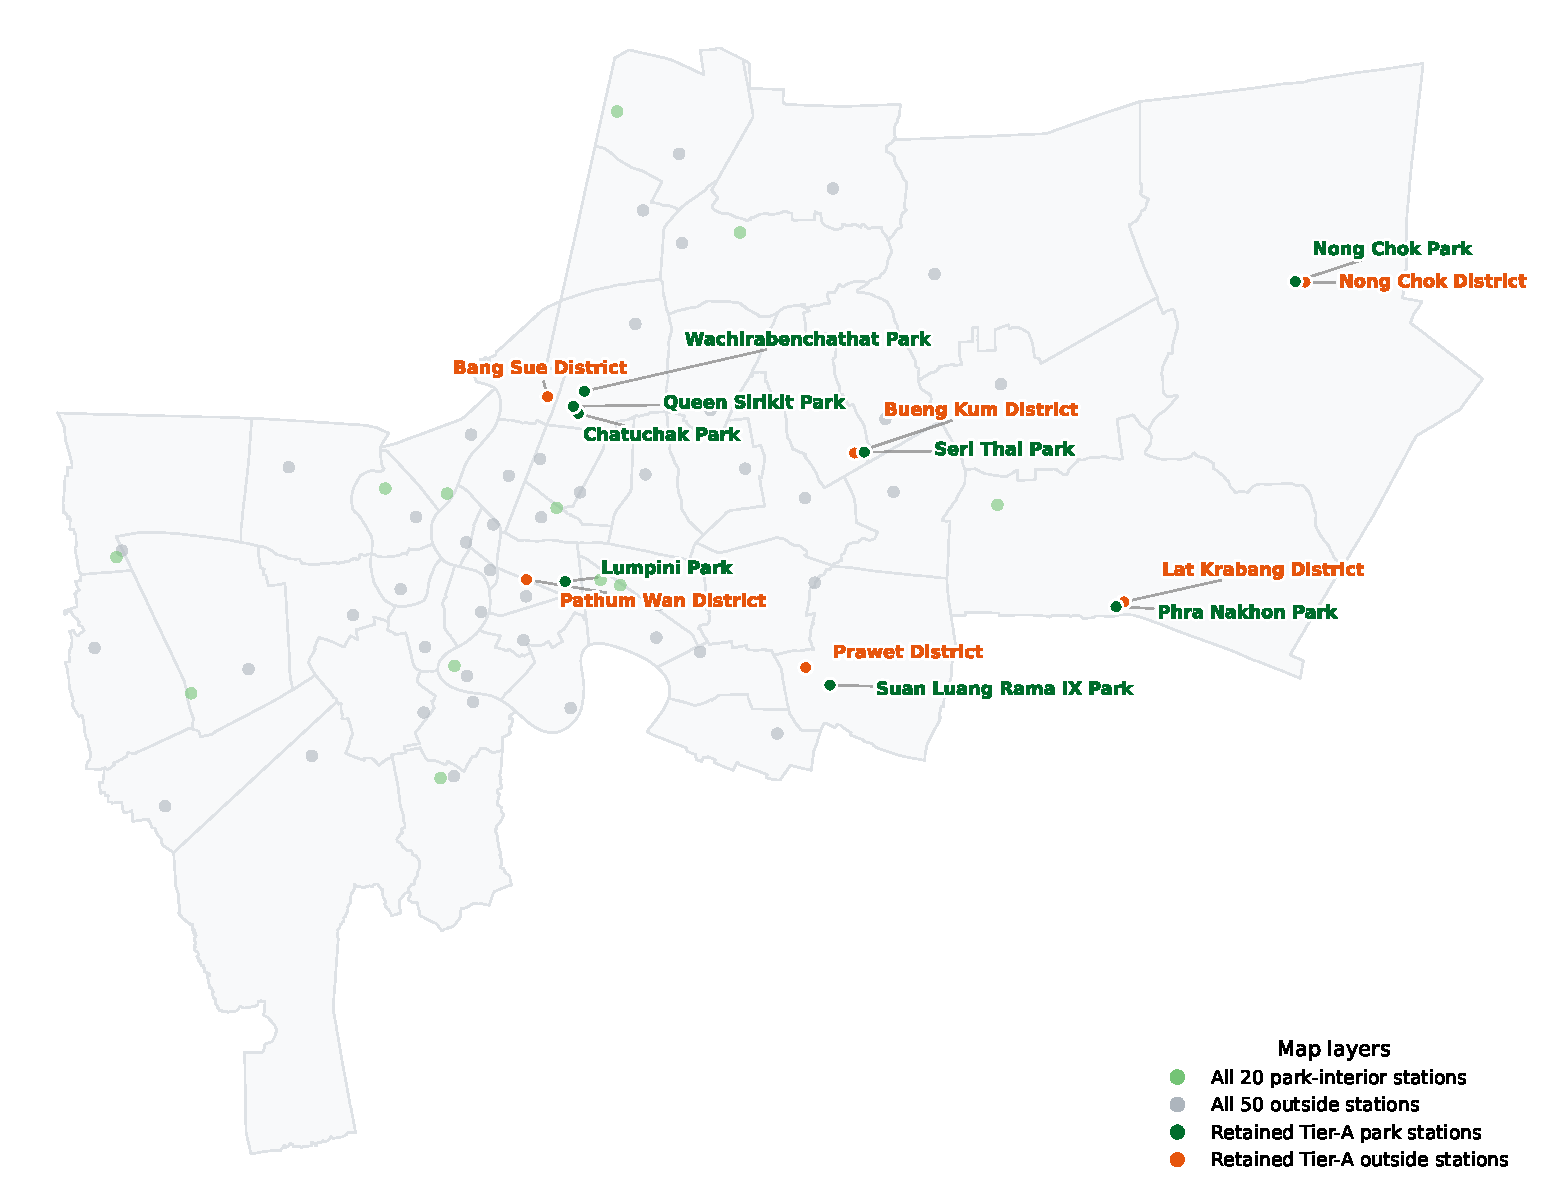
\includegraphics[width=\textwidth]{figures/Fig1_study_area_map.pdf}
\caption{Study area map of Bangkok showing the 20 park-interior PM$_{2.5}$ monitoring stations, the 50 district-level outside stations, and the eight retained Tier-A park--outside pairs used in the defensible 2021 wavelet analysis.}
\label{fig:study_area_map}
\end{figure}

The main contribution of this study is therefore methodological as well as substantive. It presents a transparent wavelet attenuation--coherence framework for paired urban PM$_{2.5}$ series under strict data-quality control, demonstrates that parks can be grouped into distinct damping regimes rather than treated as a single homogeneous class, and explores a layered explanatory hierarchy that extends beyond mean greenness to annulus-based land-cover gradients, water context, and morphology. By doing so, the study reframes the role of urban parks from a simple question of whether they reduce PM$_{2.5}$ on average to a more nuanced question of which parks buffer which temporal rhythms, how strongly they remain coupled to surrounding urban dynamics, and what spatial characteristics are most consistently associated with those outcomes.
\section{Materials and Methods}

\subsection{Study area and data}

This study was conducted in Bangkok, Thailand, a large tropical metropolitan area characterized by dense urban development, heavy traffic, heterogeneous land use, and recurrent PM$_{2.5}$ episodes. The analysis was intentionally framed as a 2021 case study because this year provided the most defensible full-year station pairing after quality control and overlap screening. Later years were examined separately for replication potential, but they did not satisfy the same annual data-quality requirements and were therefore excluded from the main wavelet analysis.

The PM$_{2.5}$ dataset comprised two monitoring groups: 20 park-interior stations and 50 district-level outside stations distributed across Bangkok. Hourly air-quality and co-located meteorological observations were provided by the Pollution Control Department (PCD), Ministry of Natural Resources and Environment (MONRE), Thailand, through its air-quality management division, for monitoring stations in Bangkok. Hourly observations were used as the common temporal resolution for all subsequent processing steps. The park-interior series were treated as the focal ``inside'' records, while the district-level stations served as candidate ``outside'' comparators for paired analysis.

English park and district names were standardized from the original Thai station filenames. Where a widely recognized English name was available, that form was used; otherwise, a consistent transliteration from Thai was retained.

To support the explanatory spatial analysis, Sentinel-2 Level-2A surface reflectance imagery for 2021 \citep{Drusch2012} was used to derive land-cover indices around park and outside stations. The primary spectral products included the Normalized Difference Vegetation Index (NDVI) \citep{Tucker1979} and the Normalized Difference Built-up Index (NDBI) \citep{Zha2003}. In the later explanatory extension, water-related indices were also included, specifically the Normalized Difference Water Index (NDWI) \citep{McFeeters1996} and the Modified Normalized Difference Water Index (MNDWI) \citep{Xu2006}. Station-centered buffer and annulus summaries were derived from these spatial layers to quantify park--outside contrast across multiple spatial scales.

Park boundary polygons were used to characterize park morphology. Candidate park polygons were obtained from OpenStreetMap-derived sources and linked to the station locations, after which a focused manual quality-control review was carried out for the 8 main wavelet parks. Candidate summaries, candidate maps, and an editable QC table were prepared for these parks, and the reviewed polygon selections were then applied to generate the final reviewed polygon set used for morphology extraction. These polygons supported the derivation of structural descriptors intended to move beyond simple mean greenness and toward a more spatially explicit description of park form. Final morphology-based interpretation was restricted to the main 2021 analysis framework and was treated as exploratory rather than causal.

\subsection{Data preprocessing and quality control}

The park PM$_{2.5}$ workflow began with filename standardization, spreadsheet ingestion, and conversion to hourly station-level time series. Unphysical negative PM$_{2.5}$ values were set to missing, while potential spikes were audited but not automatically deleted. Each park record was then placed on a fixed hourly grid covering the full 2021 calendar year (8760 hours), with missingness preserved explicitly rather than hidden by aggressive gap filling.

The outside-station PM$_{2.5}$ data were processed using a parallel hourly-cleaning workflow. The main objective at this stage was not to maximize the number of usable stations, but to apply a transparent and defensible quality screen for wavelet pairing. Outside stations were therefore screened within the 2021 hourly window and classified conservatively according to data completeness and usability.

For the main wavelet analysis, an outside station was retained only if its 2021 hourly record passed the cleaning checks and contained no more than 5\% missing PM$_{2.5}$ values across the year. In practical terms, this meant that only stations with dense and stable hourly coverage were allowed to serve as outside comparators. This screen yielded six Tier-A outside stations: Pathum Wan, Bang Sue, Lat Krabang, Nong Chok, Bueng Kum, and Prawet. Stations failing this criterion were excluded from the main paired wavelet analysis, even if they retained some descriptive value for preliminary inspection. The overall quality-control, nearest-neighbor pairing, and Tier-A pair-filtering workflow is summarized in Fig.~\ref{fig:qc_flowchart}.

\subsection{Park--outside pairing and annual analysis window}

Each park was linked deterministically to candidate outside stations using nearest-station geodesic distance calculated from latitude and longitude coordinates. Pairing between park-interior and outside stations was therefore based on geographic proximity rather than on formal Bangkok administrative district boundaries or zoning rules. Accordingly, district names in the paired results are used only as outside-station location identifiers and should not be interpreted as indicating that the park and outside station belonged to the same administrative unit.

To preserve reproducibility and avoid subjective reassignment, only the nearest outside station was used for the main analysis. Parks whose nearest outside station did not meet the Tier-A quality criterion were not carried forward into the main paired wavelet stage. Under this rule, Phra Nakhon Park was paired with Lat Krabang District, which was the most geographically distant retained pairing in the sample. This reflects the combination of the nearest-neighbor rule and the Tier-A quality filter, and should be considered when interpreting that pair's regime behavior.

This rule yielded eight park--outside pairs for the defensible 2021 wavelet analysis. After hourly merging of inside and outside records, all retained pairs showed high overlap, with both-series coverage ranging from approximately 0.970 to 0.996 of the 8760-hour year. The final retained 2021 park--outside pairs are summarized in Table~\ref{tab:final_pairs_2021}.

\begin{table}[htbp]
\centering
\small
\caption{Final retained 2021 park--outside pairs used in the defensible annual wavelet analysis. District names identify outside-station locations only; pairing was based on nearest geodesic distance from latitude--longitude coordinates rather than Bangkok administrative district assignment. Coverage is reported as overlapping non-missing hours divided by the full 8760-hour year.}
\label{tab:final_pairs_2021}
\begin{tabular}{p{4.6cm}p{3.9cm}p{3.0cm}}
\toprule
Park & Outside-station location & Coverage \\
\midrule
Chatuchak Park & Bang Sue District & 8636 / 8760 (0.986) \\
Phra Nakhon Park & Lat Krabang District & 8606 / 8760 (0.982) \\
Lumpini Park & Pathum Wan District & 8722 / 8760 (0.996) \\
Wachirabenchathat Park & Bang Sue District & 8657 / 8760 (0.988) \\
Queen Sirikit Park & Bang Sue District & 8694 / 8760 (0.992) \\
Nong Chok Park & Nong Chok District & 8713 / 8760 (0.995) \\
Suan Luang Rama IX Park & Prawet District & 8665 / 8760 (0.989) \\
Seri Thai Park & Bueng Kum District & 8494 / 8760 (0.970) \\
\bottomrule
\end{tabular}
\end{table}

Missing values were retained as \texttt{NaN} during the main cleaning stages to preserve transparency. For the wavelet stage, only very small gaps of up to 3 consecutive hours were interpolated. This conservative choice was intended to stabilize local transform behavior without converting incomplete records into artificially dense time series.

\begin{figure}[htbp]
\centering
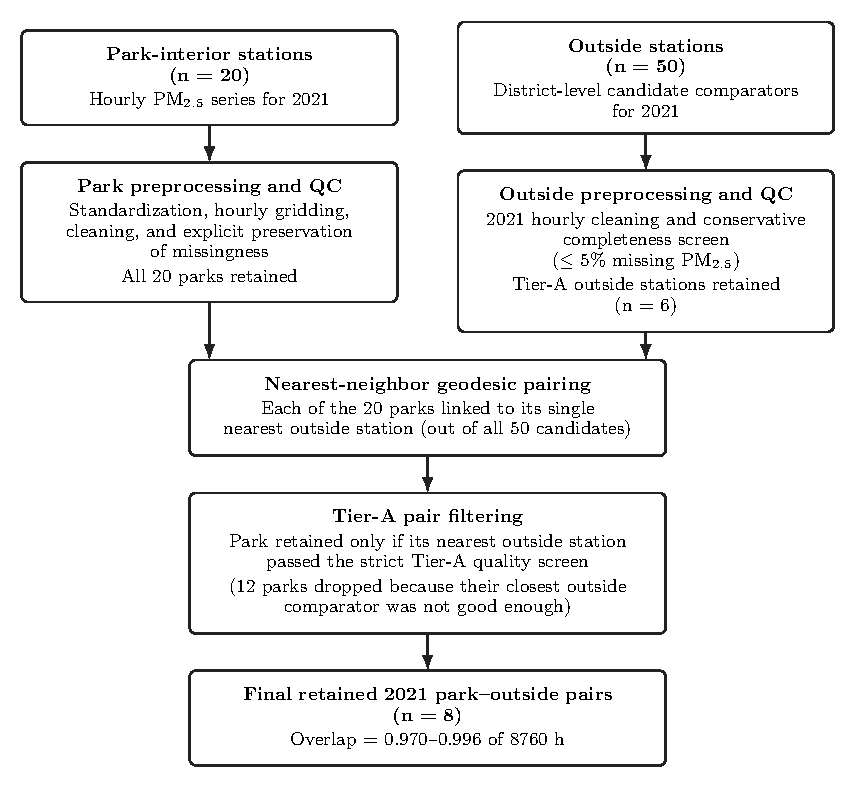
\includegraphics[width=0.92\textwidth]{figures/Fig2_qc_screening_flowchart.pdf}
\caption{Quality-control and pairing workflow for the defensible 2021 Bangkok park--outside wavelet analysis. The study began with 20 park-interior stations and 50 district-level outside stations. Park records were standardized, cleaned, and placed on a fixed 2021 hourly grid; all 20 parks remained available for pairing after this stage. Outside stations were screened more conservatively for the main wavelet analysis, and only stations with no more than 5\% missing PM$_{2.5}$ values in the 2021 hourly record were retained as Tier-A outside comparators. Each park was then linked to its single nearest outside station from among all 50 candidates by geodesic distance; pairs were retained only if the nearest outside station had independently passed the Tier-A quality screen, yielding eight final park--outside pairs with high overlapping annual coverage.}
\label{fig:qc_flowchart}
\end{figure}

\subsection{Wavelet attenuation and coherence framework}

Timescale-specific PM$_{2.5}$ behavior was quantified using a continuous wavelet transform (CWT) framework applied to each paired hourly series. The implementation was carried out in Python using the PyWavelets library (\texttt{pywt.cwt}). For the attenuation analysis, wavelet power was derived using the built-in real Morlet wavelet (\texttt{"morl"}). For the coherence analysis, a complex Morlet wavelet (\texttt{"cmor1.5-1.0"}) was used so that the cross-wavelet product and coherence surface were computed from complex-valued coefficients. Target periods were defined on an hourly grid from 2 h to 14 d, and scales were obtained by converting period in samples to wavelet scale using the PyWavelets central frequency for the corresponding wavelet family. The purpose was to decompose the park and outside records into comparable temporal bands so that attenuation and coherence could be evaluated as functions of timescale rather than as single time-averaged differences.

Wavelet attenuation was defined from the ratio of inside to outside wavelet power:
\[
\mathrm{Attenuation\ (dB)} = 10 \log_{10}\left(\frac{P_{\mathrm{in}}}{P_{\mathrm{out}}}\right),
\]
where $P_{\mathrm{in}}$ and $P_{\mathrm{out}}$ denote the park-interior and outside wavelet power, respectively. Negative values indicate damping of PM$_{2.5}$ variability inside the park relative to the outside comparator, whereas positive values would indicate amplification. The analysis window covered periods from 2 h to 14 d. In the main analysis, a fixed 24-h boundary trim was applied before wavelet summarization to reduce edge effects. Because a fixed trim does not fully remove long-period cone-of-influence exposure, an additional sensitivity check was performed using a stricter 14-day trim at both ends of the series.

For interpretation, attenuation and coherence were summarized within five predefined period bands, defined exactly in hours as 2--6 h, 6--18 h, 18--30 h (diurnal), 48--168 h (2--7 d), and 168--336 h (7--14 d). These bands were selected to separate short-term fluctuations, sub-diurnal variability, the daily rhythm, and broader multi-day behavior relevant to urban pollution episodes.

For cross-pair summaries, attenuation was reported primarily using the median across the eight retained pairs in order to reduce sensitivity to extreme park-level values, whereas coherence was summarized using the mean because it is bounded between 0 and 1 and showed less extreme dispersion across pairs. This difference in summary metric was adopted to preserve robustness for attenuation while retaining straightforward interpretability for coherence.

Wavelet coherence was used to quantify the degree to which park and outside records remained dynamically coupled at each timescale \citep{Grinsted2004}. Coherence was computed from the complex cross-wavelet product and summarized as a smoothed $R^2(s,t)$ surface, obtained as the squared magnitude of the smoothed cross-wavelet term divided by the product of the smoothed individual wavelet-power terms. Smoothing was implemented as a separable moving-average operation with reflect padding to preserve matrix size, using a 24-h window along the time axis and a 3-bin window along the scale axis. The resulting coherence values were bounded to the interval $[0,1]$ before band averaging. No formal significance test was applied, so the coherence analysis is interpreted descriptively rather than as a significance-thresholded detection framework. High coherence indicates that the park and outside station share similar temporal organization at a given band, even if their amplitudes differ, whereas lower coherence suggests temporal decoupling.

Together, attenuation and coherence provide a more informative paired framework than mean concentration comparison alone. A park may reduce the amplitude of PM$_{2.5}$ variability while still preserving the timing of broader urban oscillations, or it may both damp and decouple from the outside signal. This joint interpretation forms the basis for the regime classification developed later in the Results and Discussion sections.

The overall wavelet-analysis workflow used to derive attenuation and coherence metrics is summarized in Fig.~\ref{fig:wavelet_framework}.

\begin{figure}[htbp]
\centering
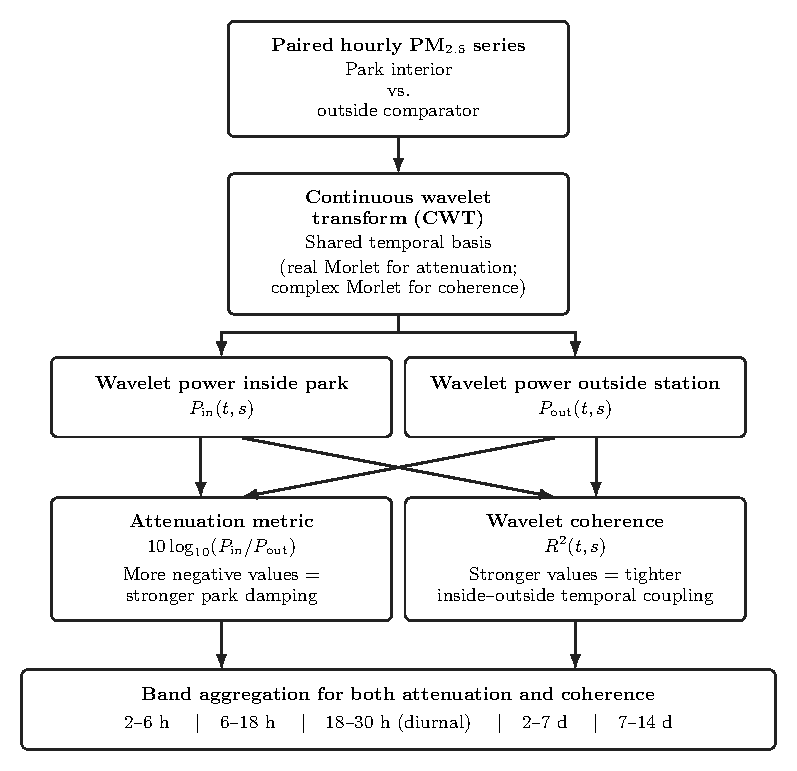
\includegraphics[width=\textwidth]{figures/Fig3_wavelet_framework_schematic.pdf}
\caption{Conceptual wavelet-analysis workflow used for paired 2021 park--outside PM$_{2.5}$ series. Hourly PM$_{2.5}$ records from each park-interior station and its paired outside comparator were transformed into the wavelet domain to obtain timescale-resolved power and coherence information. Inside/outside power ratios were converted to attenuation in decibels, while wavelet coherence was used to quantify the strength of temporal coupling between the two series. Both attenuation and coherence were then aggregated into five predefined bands: 2--6 h, 6--18 h, 18--30 h, 2--7 d, and 7--14 d.}
\label{fig:wavelet_framework}
\end{figure}

\subsection{Spatial explanatory features}

To investigate why some parks displayed stronger damping behavior than others, the study used a layered set of explanatory predictors derived from remote sensing and park geometry. The first layer consisted of station-centered Sentinel-2 indices extracted for both park and outside stations. For the 2021 land-cover stage, NDVI and NDBI were derived from the Sentinel-2 Level-2A surface-reflectance product \texttt{COPERNICUS/S2\_SR\_HARMONIZED} \citep{Drusch2012} over the period 2021-01-01 to 2022-01-01. Scenes were filtered to \texttt{CLOUDY\_PIXEL\_PERCENTAGE < 60}, and a conservative Scene Classification Layer (SCL)-based mask was applied to retain classes 4, 5, 6, and 7 before yearly compositing. NDVI was computed from bands B8 and B4 \citep{Tucker1979}, and NDBI from bands B11 and B8 \citep{Zha2003}. A yearly median composite was then formed, and buffer means were extracted at 10 m resolution for 250, 500, and 1000 m station-centered buffers around both park and outside locations. These products were then transformed into paired contrast variables such as $\Delta$NDVI and $\Delta$NDBI, defined as park minus outside values.

The explanatory framework was then extended from simple mean buffers to annulus-based spatial structure. This was motivated by the possibility that PM$_{2.5}$ buffering depends not only on average greenness, but also on how vegetation and built surfaces are organized radially around the station. Annulus-based summaries were therefore used to characterize ring-gradient patterns around both park and outside locations, allowing the analysis to test whether spatial structure outperformed simple mean land-cover indicators.

A water-related explanatory layer was added later using NDWI \citep{McFeeters1996} and MNDWI \citep{Xu2006}, together with related buffer- and annulus-based water-context summaries. These metrics were intended to capture whether nearby water or moisture-related land-cover structure contributed additional explanatory value beyond vegetation and built-up contrast alone. Because this component was developed after the core wavelet stage, it is treated as a strengthening extension to the 2021 explanatory framework rather than as an independent primary dataset.

A final structural layer described park morphology using polygon-based metrics. These morphology variables were intended to capture aspects of park form that are invisible to mean spectral indices, such as size, shape, compactness, and the potential existence of protected interior space. The explanatory analysis was therefore explicitly multi-layered: mean land cover, ring gradients, water context, and morphology were evaluated as complementary rather than competing descriptions of park buffering context.

\subsection{Exploratory association scans and robustness logic}

Associations between explanatory features and wavelet outcomes were evaluated using exploratory rank-based statistics. The main objective was not formal prediction from a large sample, but rather transparent identification of candidate relationships between spatial structure and timescale-specific damping behavior across the eight defensible 2021 pairs.

Spearman correlation was used to scan relationships between explanatory variables and band-specific attenuation or coherence metrics. The scan was expanded across multiple buffers and feature families, and initial interpretation focused on the strongest absolute correlation values rather than on null-hypothesis significance alone. This was necessary because the effective sample size for pair-level inference was small ($n = 8$), making all statistical findings necessarily exploratory.

To reduce the risk that a single park dominated interpretation, a leave-one-out robustness check was applied to the main land-cover relationship scan. Under this approach, each pair was removed in turn and the correlation recomputed, allowing the stability of candidate relationships to be inspected across all eight leave-one-out subsets. This step was included primarily as reviewer-oriented robustness logic rather than as proof of causality.

Additional annual replication screening was conducted for 2022 and 2023 to test whether the 2021 framework could be extended directly across years. Under the same conservative annual completeness logic used to define defensible outside comparators for 2021, the later-year outside series were found to be too sparse and fragmented for defensible annual wavelet replication. The main manuscript is therefore intentionally framed as a rigorous 2021 Bangkok case study rather than a multi-year annual comparison.
\section{Results}

\subsection{Wavelet attenuation: parks damp PM$_{2.5}$ variability}

Across the eight retained 2021 park--outside pairs, attenuation was negative overall, indicating that park interiors consistently reduced PM$_{2.5}$ variability relative to their paired outside comparators. This damping was not uniform across timescales. The strongest attenuation occurred at multi-day scales, with median band-mean attenuation of approximately $-8.0$ dB at 2--7 d and $-7.5$ dB at 7--14 d. Damping was also clearly expressed at sub-diurnal scales, with a median of approximately $-6.3$ dB at 6--18 h. The diurnal band (18--30 h) was the least damped, with a median of approximately $-3.8$ dB. The shortest band (2--6 h) was slightly more negative (about $-4.2$ dB median) but showed greater pair-to-pair variability. Thus, attenuation strengthened from 2--6 h to 6--18 h, dipped at the diurnal band, and then intensified again at multi-day scales. Overall, these results indicate that Bangkok parks buffered PM$_{2.5}$ variability most effectively at sub-diurnal and multi-day timescales, while the daily cycle remained comparatively resistant to damping (Fig.~\ref{fig:attenuation_by_band}).

Substantial heterogeneity was evident across individual parks. At the long-period end, Nong Chok Park showed the strongest attenuation, reaching approximately $-27.4$ dB at 7--14 d, whereas Seri Thai Park showed only weak long-band damping of approximately $-1.9$ dB at the same band. Suan Luang Rama IX Park also showed strong attenuation at daily and multi-day scales, while the three northern-cluster parks paired to Bang Sue District (Chatuchak Park, Wachirabenchathat Park, and Queen Sirikit Park) exhibited consistent broadband negative attenuation of moderate magnitude. In contrast, some parks showed weak or mixed short-band behavior despite remaining clearly damped at longer timescales. This heterogeneity motivated both the regime classification and the explanatory analysis developed below. A representative strong-decoupler example from Nong Chok Park is shown in Fig.~\ref{fig:nongchok_representative_scalograms}, where the park-interior and outside wavelet-power fields can be compared directly across the predefined bands.

\begin{figure}[htbp]
\centering
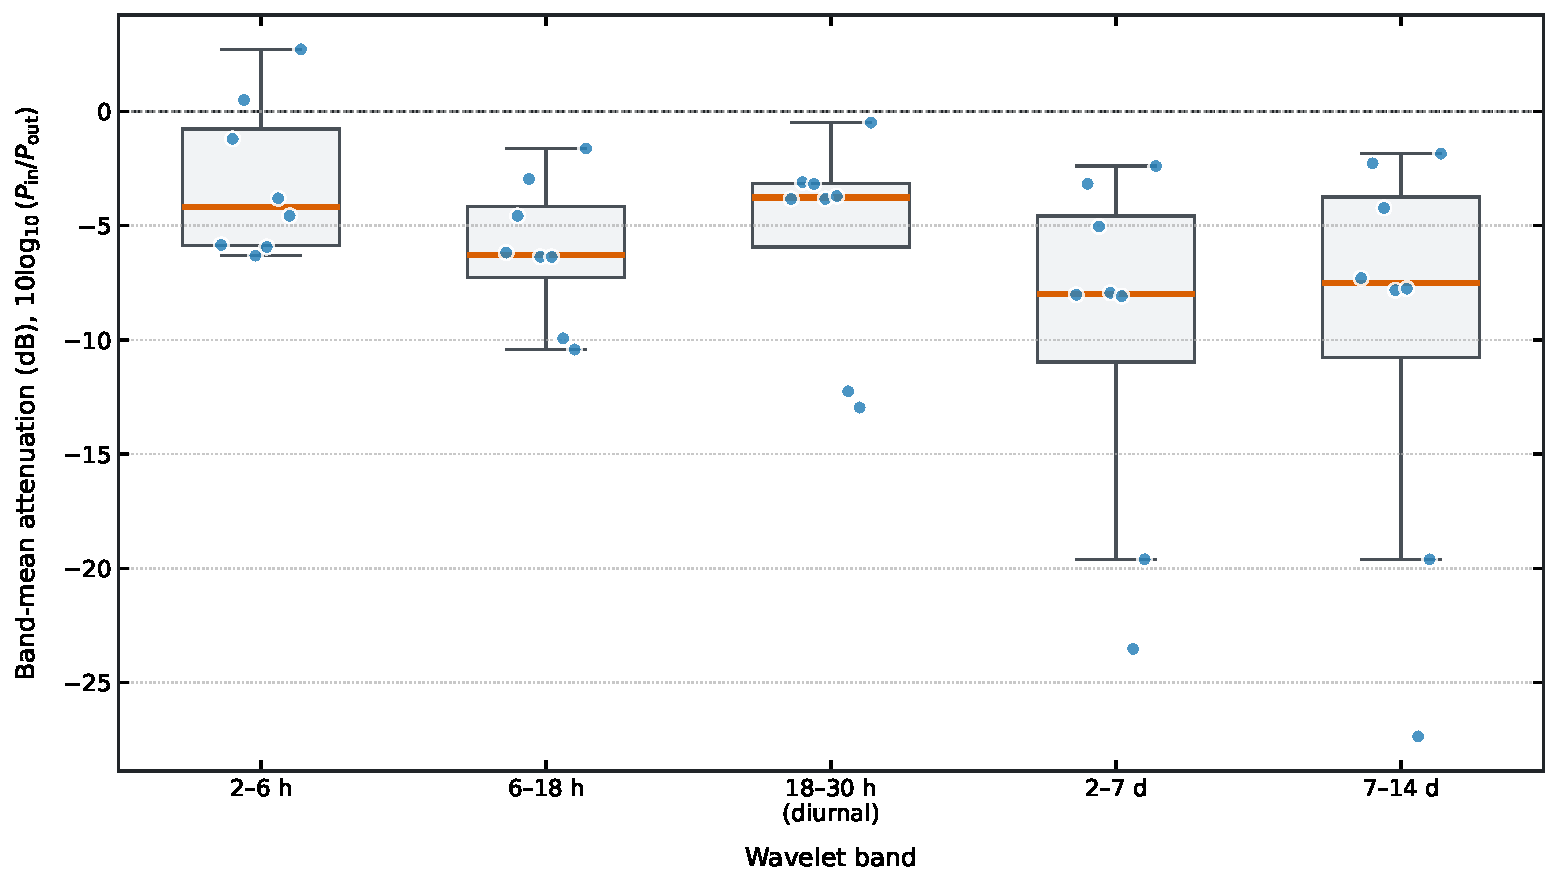
\includegraphics[width=\textwidth]{figures/Fig4_attenuation_by_band_2021.pdf}
\caption{Band-specific attenuation across the eight retained 2021 park--outside pairs. Each point represents one retained pair, while boxplots summarize the distribution within each predefined wavelet band. More negative attenuation values indicate stronger damping of park-interior PM$_{2.5}$ variability relative to the paired outside reference station. The dashed line at 0 dB marks equal variability between park and outside.}
\label{fig:attenuation_by_band}
\end{figure}

\begin{figure}[htbp]
\centering
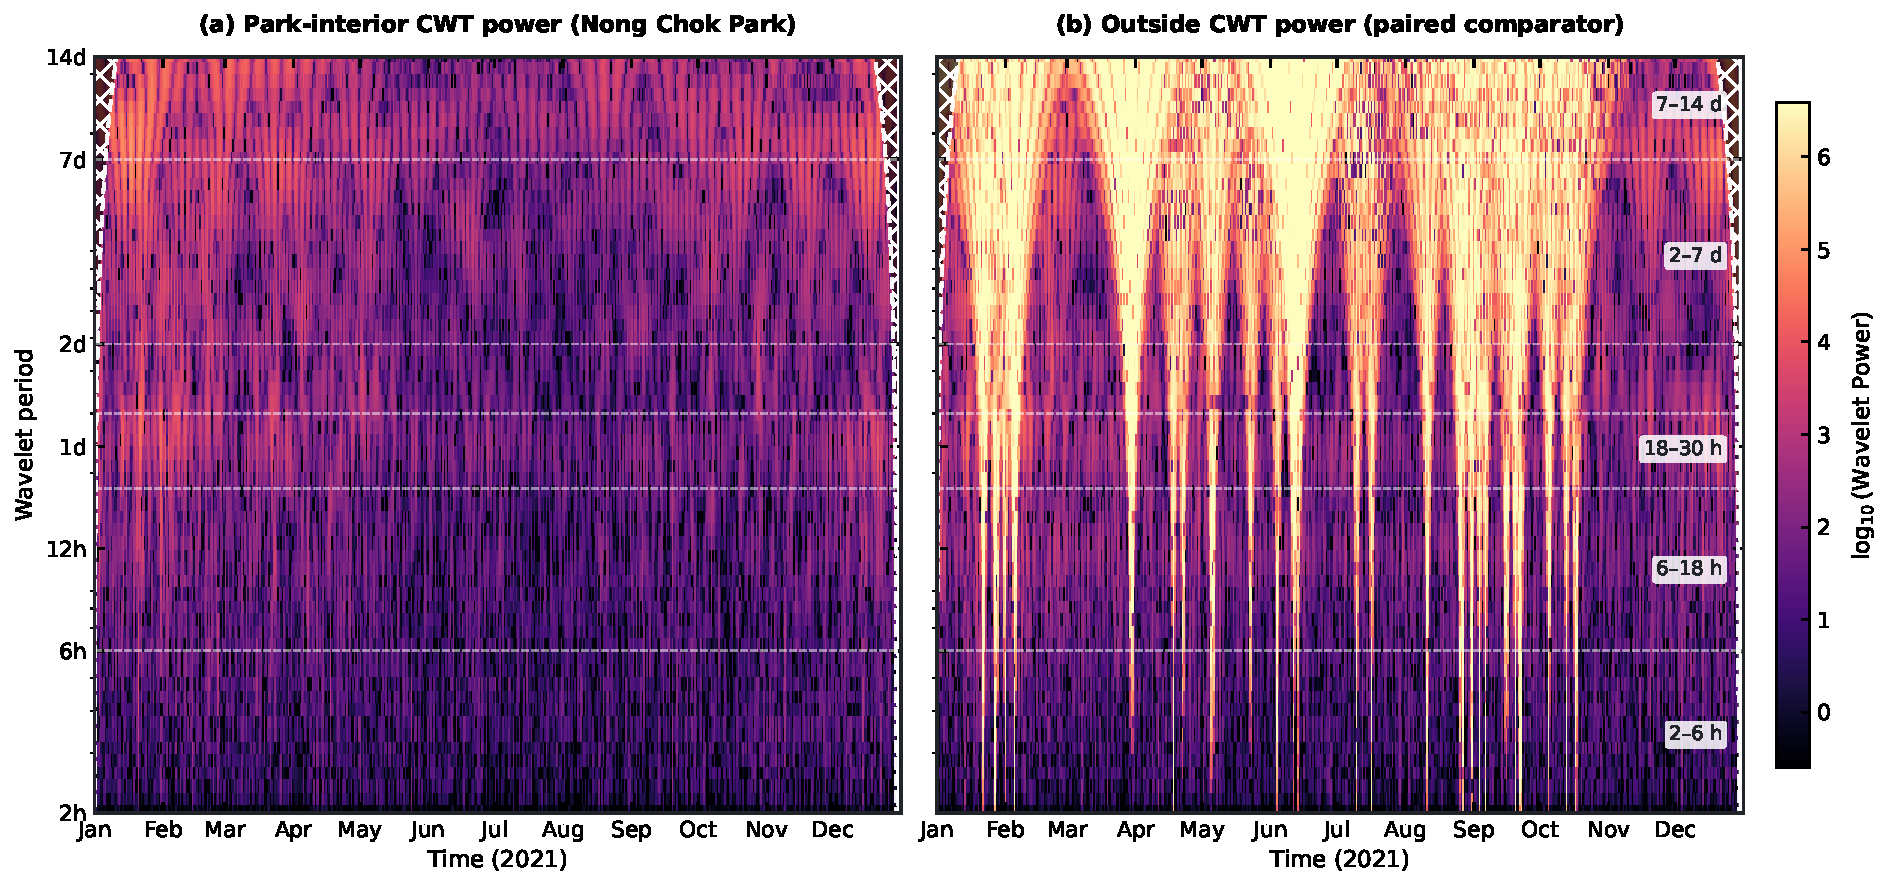
\includegraphics[width=\textwidth]{figures/Fig6_nongchok_representative_scalograms.pdf}
\caption{Representative wavelet-power example for the Nong Chok Park pair, shown here as a strong decoupler. Panel (a) shows park-interior CWT power and panel (b) shows CWT power for the paired outside comparator. Dashed horizontal lines indicate the predefined wavelet-band boundaries used in the main analysis. The hatched region below the dashed cone-of-influence (COI) curve indicates edge-affected areas that should be interpreted cautiously. The COI shown here is the native wavelet COI and therefore extends much farther than the fixed 24-h boundary trim used in the main summaries; long-period sensitivity to this choice was evaluated separately using a stricter 14-day trim.}
\label{fig:nongchok_representative_scalograms}
\end{figure}

\subsection{Wavelet coherence: parks preserve shared urban rhythms}

Wavelet coherence increased markedly from short to longer timescales. Mean coherence was approximately 0.27 at 2--6 h, 0.58 at 6--18 h, 0.78 at the diurnal band, and 0.74 at 2--7 d, before declining to about 0.57 at 7--14 d. Thus, although parks damped PM$_{2.5}$ amplitude, they did not behave as isolated atmospheric islands. Instead, park interiors generally remained embedded within broader city-scale temporal rhythms, especially at the diurnal and 2--7 d bands, with weaker coupling again at 7--14 d (Fig.~\ref{fig:coherence_by_band}).

At short periods, coherence was lower and locally variable, implying that fast fluctuations were more weakly synchronized between parks and their outside comparators than longer-timescale behavior. At diurnal and multi-day scales, coherence became consistently high, with the strongest shared timing evident at the diurnal and 2--7 d bands and lower coherence again at 7--14 d. In other words, Bangkok parks tended to flatten the signal more than they shifted its timing. This remains a more nuanced finding than a simple reduction in mean PM$_{2.5}$ concentration, because it shows that amplitude damping and temporal coupling are related but not identical dimensions of park performance.

\begin{figure}[htbp]
\centering
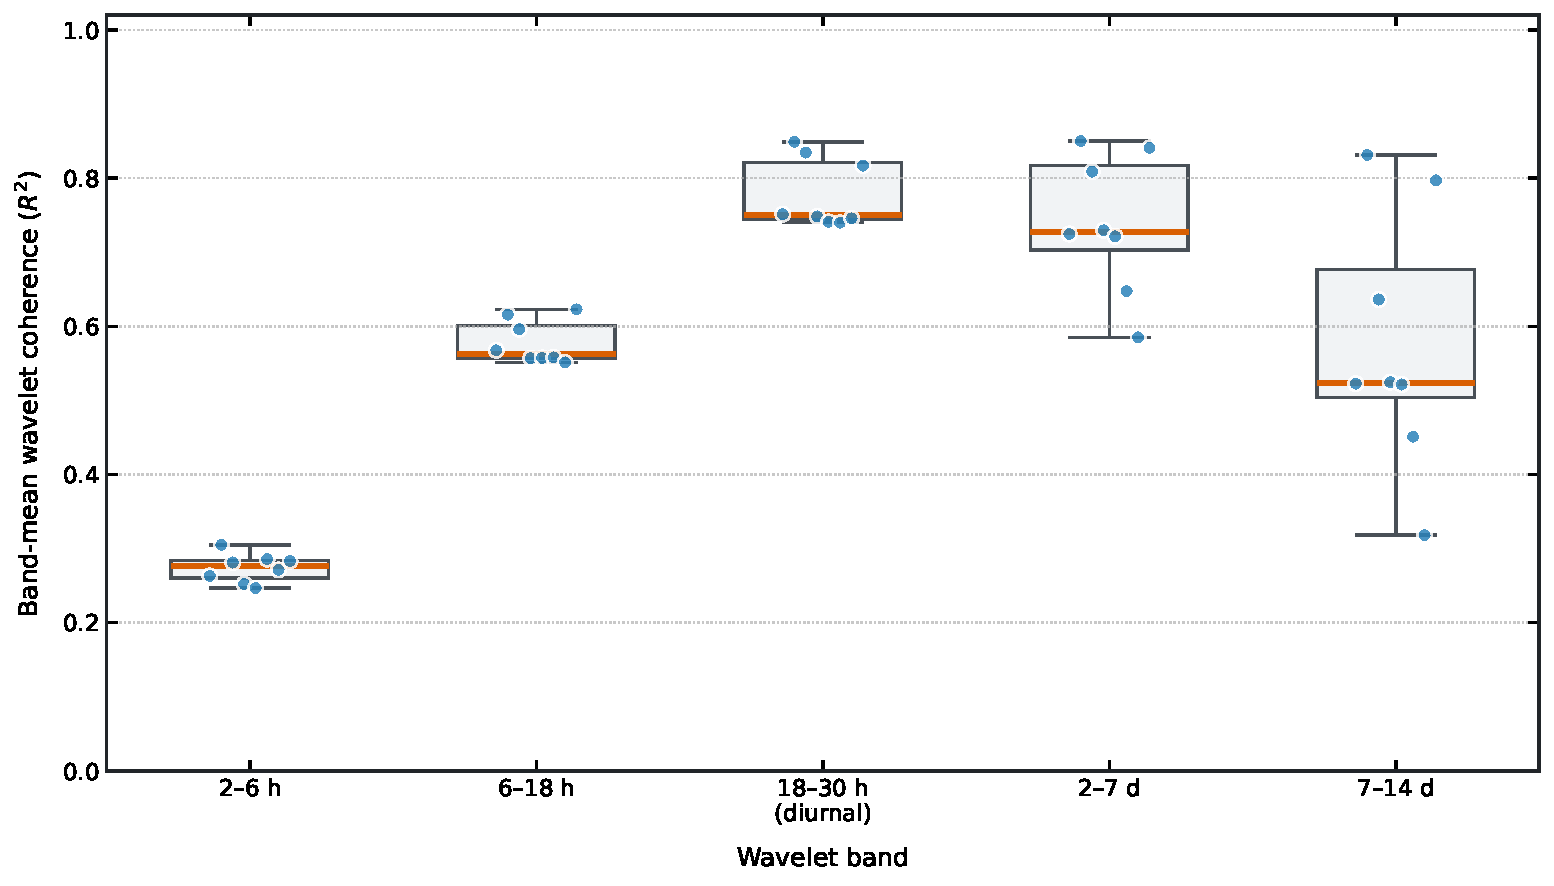
\includegraphics[width=\textwidth]{figures/Fig5_coherence_by_band_2021.pdf}
\caption{Band-specific wavelet coherence across the eight retained 2021 park--outside pairs. Each point represents one retained pair, while boxplots summarize the distribution within each predefined wavelet band. Higher coherence indicates stronger temporal coupling between park-interior and outside PM$_{2.5}$ variability at the corresponding timescale.}
\label{fig:coherence_by_band}
\end{figure}
% [Figure 2C near here: mean attenuation vs. mean coherence for each pair]

\subsection{Three park damping regimes}

When attenuation and coherence were interpreted jointly, the eight retained pairs could be organized into three distinct regimes. The first group comprised \textit{strong decouplers}, represented by Nong Chok Park and Suan Luang Rama IX Park. These parks combined very strong attenuation, especially at daily and multi-day scales, with relatively lower long-band coherence than the rest of the sample. They therefore appeared to damp PM$_{2.5}$ strongly while also partially breaking away from the surrounding urban temporal rhythm.

The second group comprised \textit{moderate broadband dampers}, represented by Chatuchak Park, Wachirabenchathat Park, and Queen Sirikit Park. These parks showed consistently negative attenuation across nearly all bands, but without the extreme long-band decoupling seen in the strongest two cases. Their behavior suggests a more stable, broadband dampening role: they reduced variability across multiple timescales while maintaining moderate synchrony with the outside urban signal.

The third group comprised \textit{weak followers or mixed cases}, represented by Phra Nakhon Park, Lumpini Park, and Seri Thai Park. These parks still showed negative attenuation overall, but their damping was weaker and their coherence remained relatively high, particularly at diurnal and multi-day scales. In practical terms, they tended to follow the outside dynamics more closely than the first two groups. This regime classification is important because it shows that parks within the same city cannot be treated as a single homogeneous class of PM$_{2.5}$ buffers, and the separation of the three groups in mean attenuation--mean coherence space is visualized in Fig.~\ref{fig:regime_scatter}.

A second implication of the regime concept is that park buffering performance should not be interpreted through one scalar summary alone. For example, two parks may have similarly low mean PM$_{2.5}$ but very different temporal signatures: one may act as a strong decoupler that suppresses multi-day peaks, whereas another may simply track the outside station with only modest amplitude reduction. The wavelet framework therefore reveals a hierarchy of buffering behavior that would be obscured by static mean comparisons.

\begin{figure}[htbp]
\centering
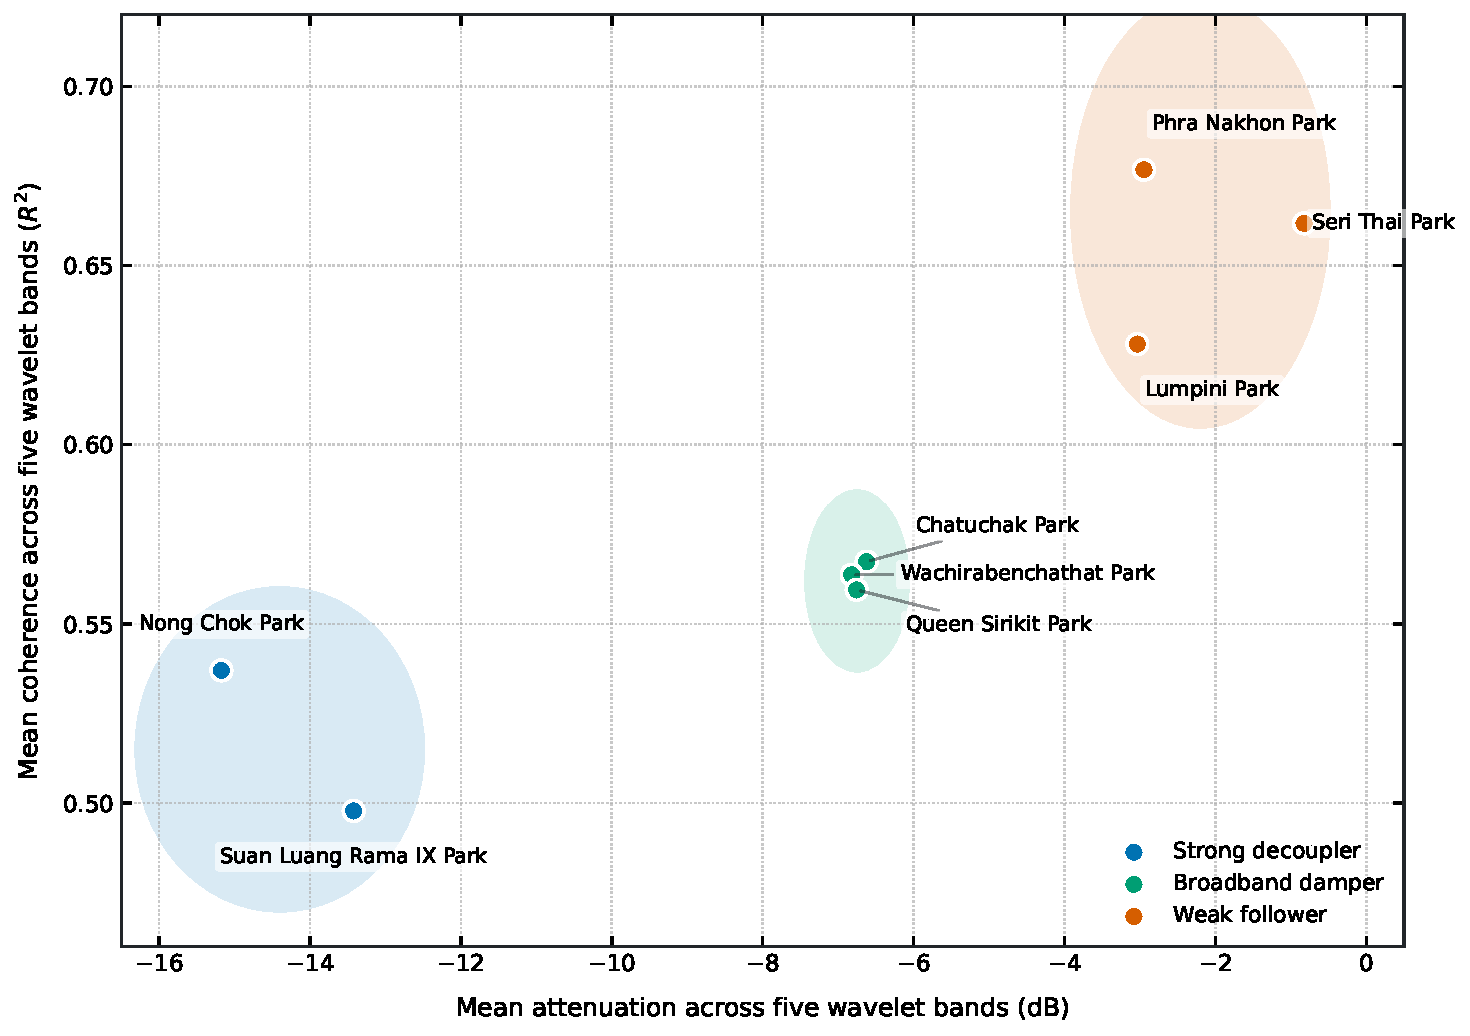
\includegraphics[width=\textwidth]{figures/Fig7_regime_scatter_mean_att_mean_coh.pdf}
\caption{Attenuation--coherence regime map for the eight retained 2021 park--outside pairs, using the mean attenuation and mean coherence aggregated across the five predefined wavelet bands. Each point represents one park pair and is labeled by park name. The shaded groupings indicate the three qualitative regimes identified in the paired wavelet analysis: strong decouplers, broadband dampers, and weak followers.}
\label{fig:regime_scatter}
\end{figure}

Table~\ref{tab:park_regime_summary} summarizes the exact band-mean attenuation and mean coherence values underlying the three-regime classification. Rows are ordered by regime so that the contrast between strong decouplers, moderate broadband dampers, and weak followers or mixed cases can be read directly from the numeric wavelet summaries.

\begin{table}[htbp]
\centering
\caption{Park-level band-mean attenuation and mean wavelet coherence for the eight Tier-A park--outside pairs retained in the 2021 Bangkok analysis. More negative attenuation values indicate stronger damping of park-interior PM$_{2.5}$ fluctuations relative to the paired outside reference station. Row shading indicates the assigned attenuation--coherence regime.}
\label{tab:park_regime_summary}
\begingroup
\setlength{\tabcolsep}{3.2pt}
\renewcommand{\arraystretch}{1.12}
\scriptsize
\resizebox{\textwidth}{!}{%
\begin{tabular}{p{3.9cm}*{10}{c}p{3.8cm}}
\toprule
& \multicolumn{5}{c}{Attenuation (dB)} & \multicolumn{5}{c}{Mean coherence ($R^2$)} & \\
\cmidrule(lr){2-6} \cmidrule(lr){7-11}
Park & 2--6 h & 6--18 h & 18--30 h & 2--7 d & 7--14 d & 2--6 h & 6--18 h & 18--30 h & 2--7 d & 7--14 d & Regime \\
\midrule

\rowcolor{regimedecoupler}
Nong Chok Park
& -3.806 & -9.936 & -12.254 & -23.529 & -27.362
& 0.29 & 0.56 & 0.74 & 0.65 & 0.45
& Strong decoupler \\

\rowcolor{regimedecoupler}
Suan Luang Rama IX Park
& -4.571 & -10.424 & -12.962 & -19.607 & -19.611
& 0.27 & 0.55 & 0.75 & 0.59 & 0.32
& Strong decoupler \\

\rowcolor{regimebroadband}
Chatuchak Park
& -5.846 & -6.179 & -3.834 & -8.026 & -7.296
& 0.26 & 0.57 & 0.75 & 0.72 & 0.52
& Moderate broadband damper \\

\rowcolor{regimebroadband}
Wachirabenchathat Park
& -6.314 & -6.365 & -3.832 & -7.941 & -7.829
& 0.25 & 0.56 & 0.75 & 0.73 & 0.52
& Moderate broadband damper \\

\rowcolor{regimebroadband}
Queen Sirikit Park
& -5.936 & -6.371 & -3.708 & -8.085 & -7.758
& 0.25 & 0.56 & 0.74 & 0.72 & 0.52
& Moderate broadband damper \\

\rowcolor{regimeweak}
Phra Nakhon Park
& -1.203 & -4.572 & -3.101 & -3.169 & -2.276
& 0.31 & 0.62 & 0.85 & 0.85 & 0.83
& Weak follower / mixed case \\

\rowcolor{regimeweak}
Lumpini Park
& 0.501 & -2.956 & -3.176 & -5.037 & -4.226
& 0.28 & 0.60 & 0.83 & 0.81 & 0.64
& Weak follower / mixed case \\

\rowcolor{regimeweak}
Seri Thai Park
& 2.713 & -1.623 & -0.489 & -2.396 & -1.850
& 0.28 & 0.62 & 0.82 & 0.84 & 0.80
& Weak follower / mixed case \\

\bottomrule
\end{tabular}%
}
\endgroup
\end{table}

% [Figure 3 near here: representative peak-flattening time-series example]

\subsection{Mean land-cover contrast provides a first-order explanation}

The first explanatory layer considered whether simple park--outside land-cover contrasts based on mean Sentinel-2 buffer summaries were associated with the observed wavelet outcomes. The strongest simple-buffer relationship was a positive association between $\Delta$NDBI at the 250 m scale and 6--18 h attenuation, with Spearman $\rho = 0.595$ ($p = 0.120$). Because both $\Delta$NDBI and attenuation can take negative values in this dataset, this positive rank association means that more negative park--outside built-up contrast was associated with more negative attenuation, that is, stronger damping. An equally strong long-band built-up signal also appeared at the 500 m scale, where $\Delta$NDBI was positively associated with 7--14 d attenuation ($\rho = 0.595$, $p = 0.120$). The strongest greenness-based mean-buffer signal was a negative association between $\Delta$NDVI at the 500 m scale and 7--14 d attenuation, with $\rho = -0.571$ ($p = 0.139$). These top mean-buffer relationships are visualized in Fig.~\ref{fig:mean_buffer_landcover_scatter}.

\begin{figure}[htbp]
\centering
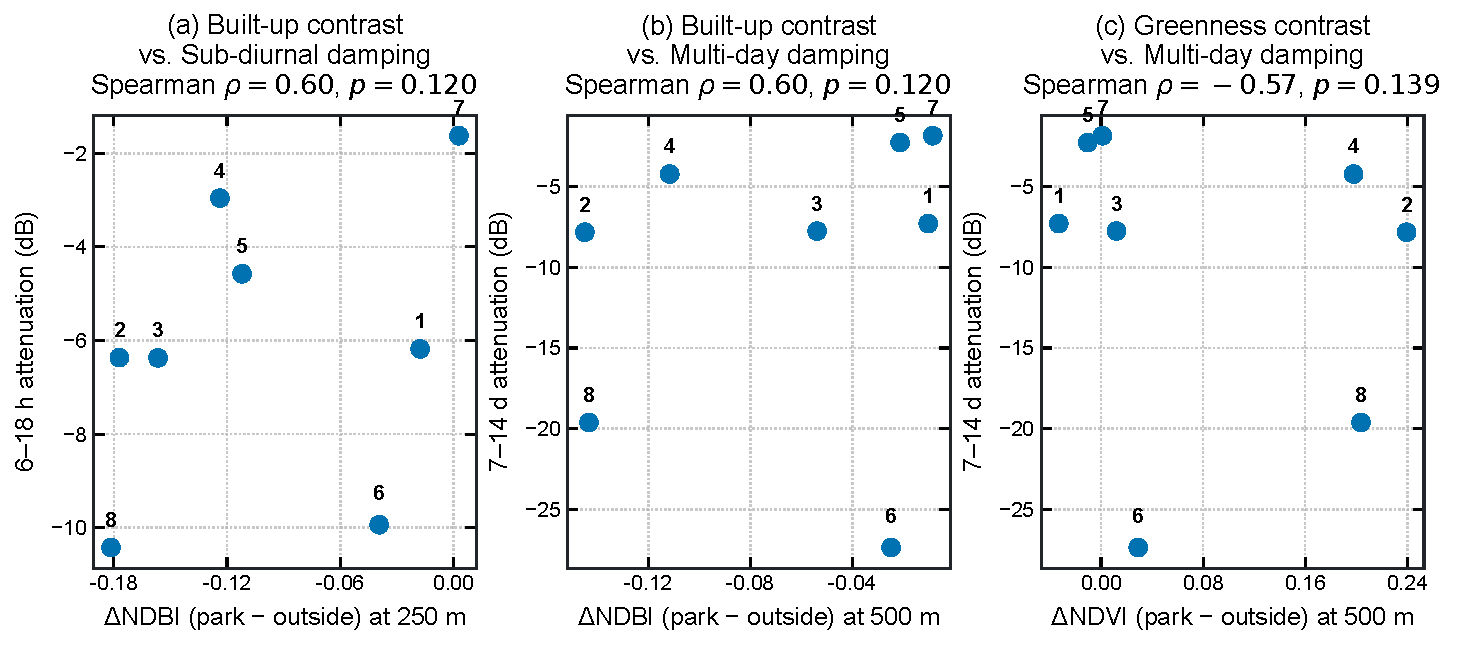
\includegraphics[width=\textwidth]{figures/Fig8_top_mean_buffer_landcover_relationships_2021.pdf}
\caption{Top mean-buffer land-cover relationships between park--outside contrasts and wavelet attenuation outcomes across the eight retained 2021 pairs.
Panels show the strongest mean-buffer associations emphasized in the Results: (i) $\Delta$NDBI at 250 m versus 6--18 h attenuation, (ii) $\Delta$NDBI at 500 m versus 7--14 d attenuation, and (iii) $\Delta$NDVI at 500 m versus 7--14 d attenuation.
Each point is one retained park--outside pair, labeled numerically as follows: 1 = Chatuchak Park (Bang Sue), 2 = Wachirabenchathat Park (Bang Sue), 3 = Queen Sirikit Park (Bang Sue), 4 = Lumpini Park (Pathum Wan), 5 = Phra Nakhon Park (Lat Krabang), 6 = Nong Chok Park (Nong Chok), 7 = Seri Thai Park (Bueng Kum), and 8 = Suan Luang Rama IX (Prawet).}
\label{fig:mean_buffer_landcover_scatter}
\end{figure}

These relationships remained directionally stable under leave-one-out testing.
For 250 m $\Delta$NDBI versus 6--18 h attenuation, the correlation remained positive across all leave-one-out subsets, ranging from $\rho = 0.393$ to $\rho = 0.821$.
For 500 m $\Delta$NDBI versus 7--14 d attenuation, the leave-one-out correlations also remained positive, ranging from $\rho = 0.393$ to $\rho = 0.786$.
For 500 m $\Delta$NDVI versus 7--14 d attenuation, the correlation remained negative throughout, ranging from $\rho = -0.714$ to $\rho = -0.464$.
Thus, although the sample size was small and the p-values should be interpreted cautiously, the sign consistency indicates that these first-order relationships were directionally robust and not solely dependent on any single park--outside pair, even though their strength varied across leave-one-out subsets.
These leave-one-out results are summarized in Fig.~\ref{fig:loo_robustness_mean_buffer}.

\begin{figure}[htbp]
\centering
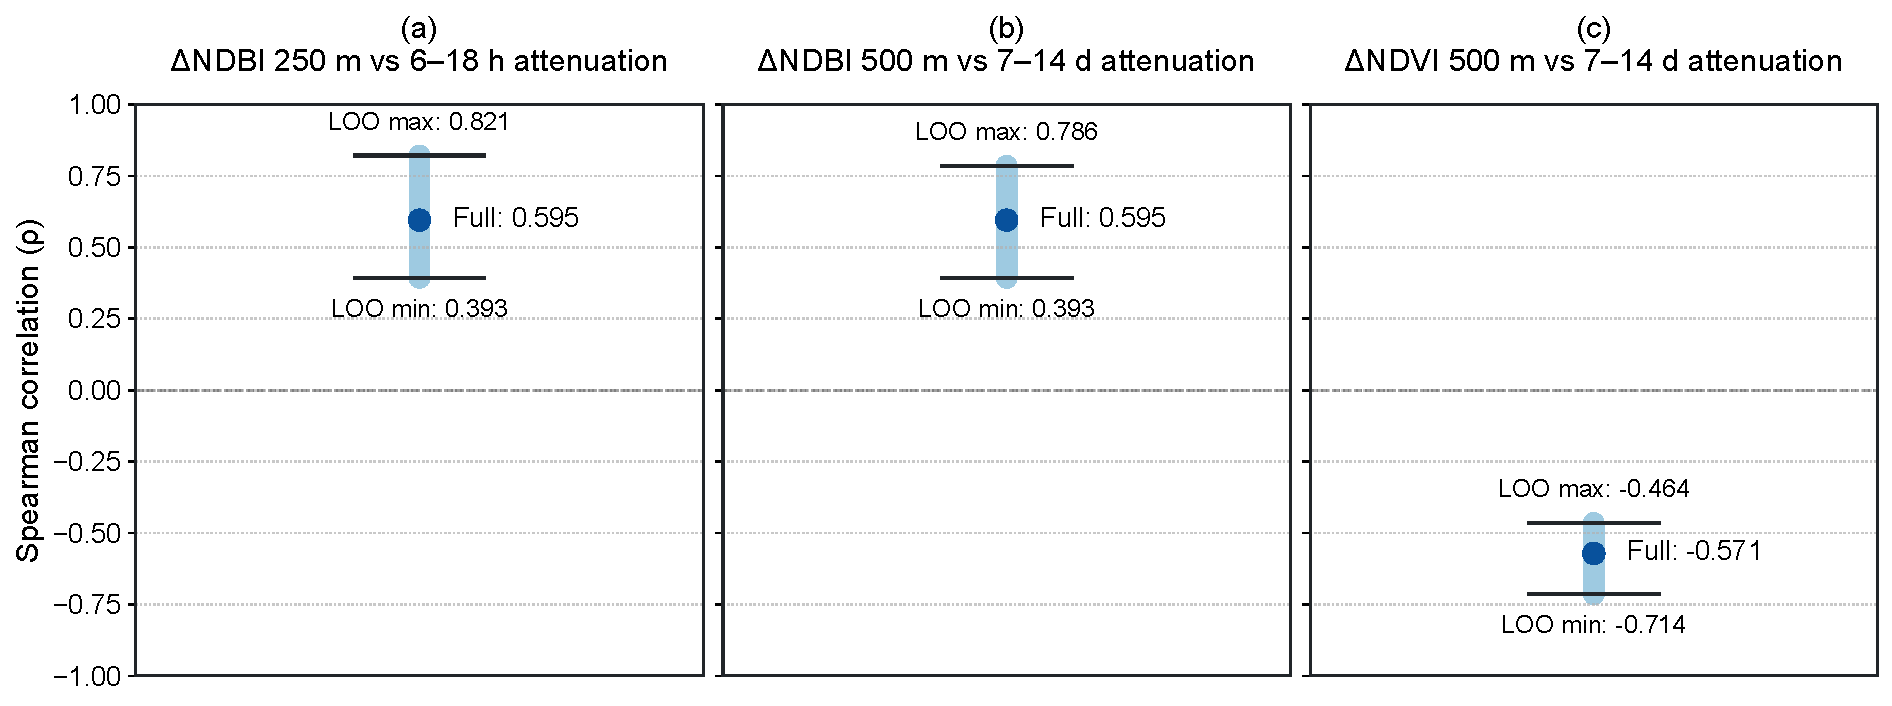
\includegraphics[width=\textwidth]{figures/Fig9_loo_robustness_mean_buffer_relationships_2021.pdf}
\caption{Leave-one-out robustness of the three leading mean-buffer land-cover relationships emphasized in the Results.
In each panel, the dark point shows the full-sample Spearman $\rho$ for the complete eight-pair dataset, while the vertical range shows the minimum and maximum $\rho$ obtained across all leave-one-out subsets.
Each leave-one-out subset contains $n=7$ pairs, obtained by dropping one park--outside pair at a time from the full eight-pair dataset.
Sign consistency across the full-sample and leave-one-out estimates indicates that the leading mean-buffer relationships are directionally robust to omission of any single pair.}
\label{fig:loo_robustness_mean_buffer}
\end{figure}

Taken together, the mean-buffer layer suggests a coherent first-order pattern: stronger park--outside built-up contrast tended to be associated with stronger attenuation, while stronger park--outside greenness contrast tended to be associated with stronger long-band damping in the opposite direction of the built-up effect.
However, these average contrasts were not sufficient to explain the full hierarchy of park behavior.
Nong Chok Park, for example, showed exceptionally strong damping without being reducible to a single mean greenness metric, while some greener parks still behaved as weaker followers.
This indicated that mean NDVI and NDBI were useful first-order descriptors, but not a complete explanatory framework on their own.

\subsection{Ring-gradient land-cover structure strengthens the explanation}

The annulus-based analysis substantially sharpened the land-cover interpretation by moving beyond cumulative mean buffers toward radial structure. In this layer, the strongest signals appeared most clearly for coherence, especially at short timescales. The contrast between the core and outer ring in outside-site NDVI showed a strong negative association with 2--6 h coherence ($\rho = -0.756$, $p = 0.030$) and with 6--18 h coherence ($\rho = -0.756$, $p = 0.030$). Conversely, the contrast between the core and outer ring in outside-site NDBI showed a strong positive association with 2--6 h coherence ($\rho = 0.708$, $p = 0.050$) and with 6--18 h coherence ($\rho = 0.708$, $p = 0.050$), with a similar but slightly weaker signal for diurnal coherence ($\rho = 0.683$, $p = 0.062$). The identical correlation values across the 2--6 h and 6--18 h bands reflect the same rank ordering of the eight retained pairs across those two coherence metrics in this small sample.

These results indicate that the radial organization around the outside comparator site mattered strongly for short-band synchrony. When the outside-site core was greener relative to its outer ring, short-band park--outside coherence tended to be lower; when the outside-site core was more built-up relative to its outer ring, short-band coherence tended to be higher. In other words, the local spatial structure of the comparator environment influenced how tightly parks remained synchronized with nearby urban fluctuations. %The strongest annulus-based relationships are visualized in Fig.~\ref{fig:annulus_ring_gradient} and summarized numerically in Table~\ref{tab:annulus_top_correlations}.

The annulus analysis also contributed to the attenuation interpretation, although these signals were somewhat weaker than the coherence results. Park--outside built-up contrast in the 250--500 m ring was positively associated with 7--14 d attenuation ($\rho = 0.619$, $p = 0.102$), while the related mid-ring built-up advantage metric showed the corresponding negative association ($\rho = -0.619$, $p = 0.102$). Similar though slightly weaker patterns appeared for long-band coherence. Taken together, these results support the idea that green-core advantage, built-edge pressure, and contrast persistence provide a better explanation of park buffering behavior than simple average greenness alone.

A key implication is that park performance was relational rather than purely internal. The strongest spatial signals were not limited to the park itself; they also depended on the radial structure of the outside comparator site. This is a central result of the study: PM$_{2.5}$ damping by parks depends not only on whether a park is green, but also on how the surrounding urban landscape is organized around both members of the pair.

\begin{figure}[htbp]
\centering
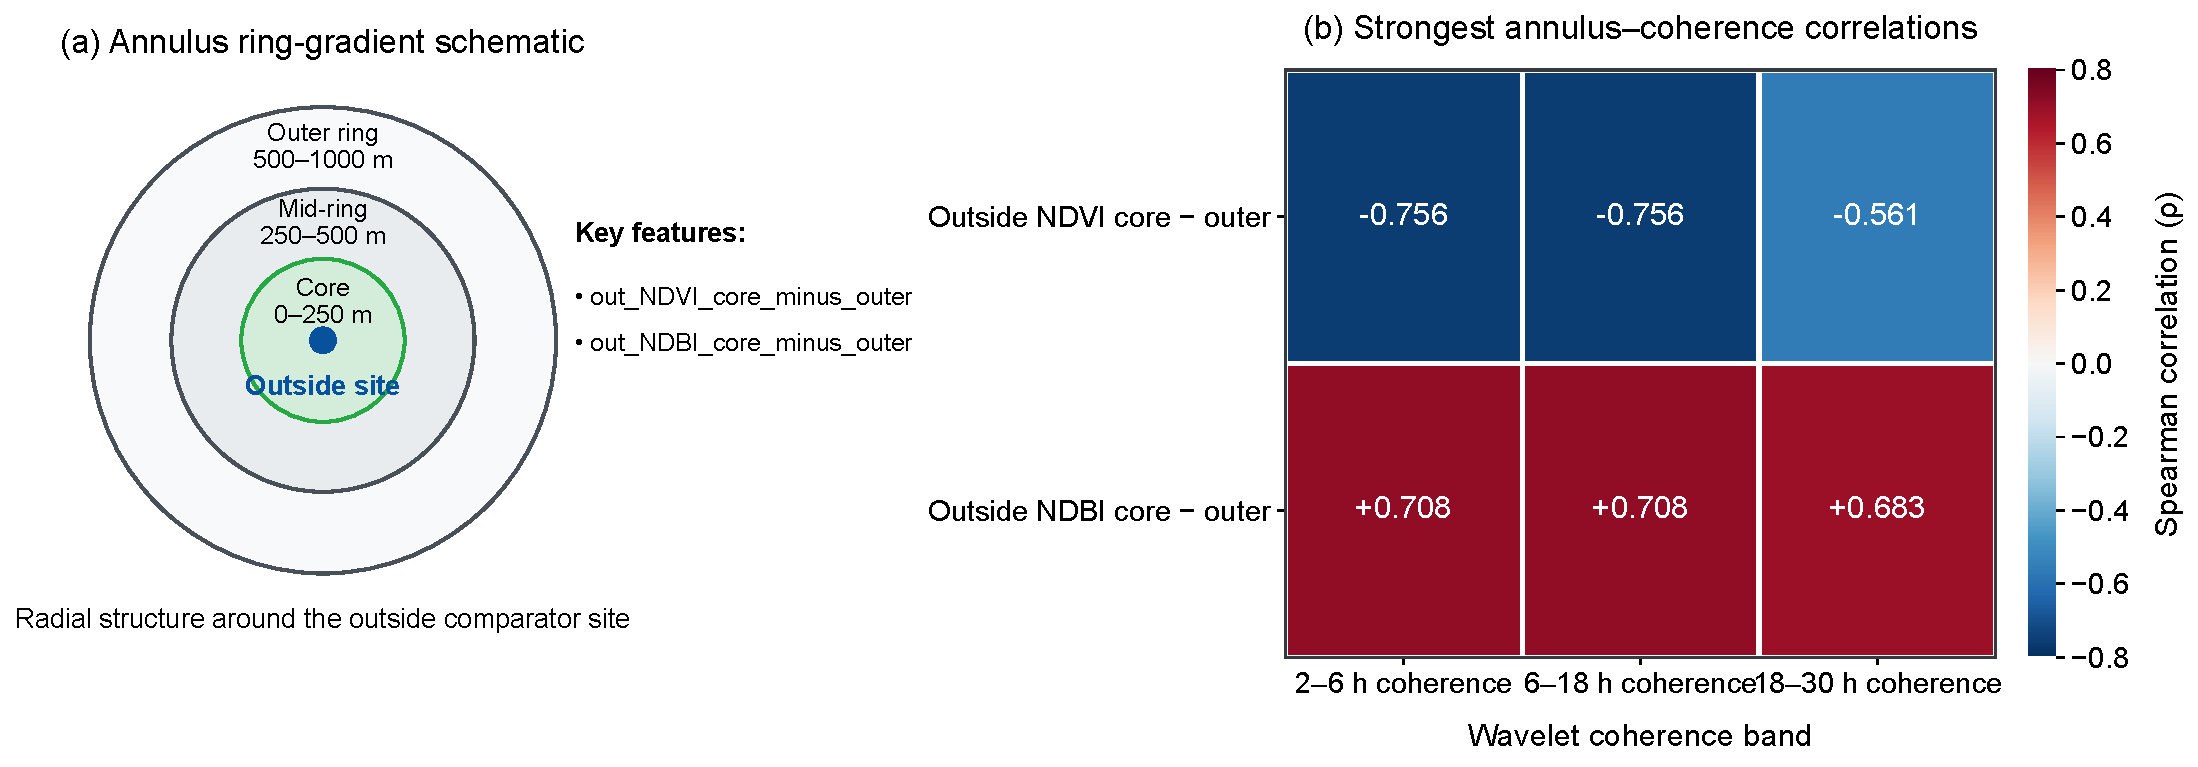
\includegraphics[width=\textwidth]{figures/Fig10_annulus_ring_gradient_schematic_results_2021}
\caption{Annulus-based ring-gradient interpretation of the strongest outside-site land-cover structure signals across the eight retained 2021 park--outside pairs. (a) Schematic of the annulus framework around the outside comparator site, showing the core (0--250 m), mid-ring (250--500 m), and outer ring (500--1000 m). The key gradients emphasized here are the core-minus-outer contrasts for outside-site NDVI and NDBI. (b) Spearman correlations between these outside-site core-minus-outer annulus contrasts and wavelet coherence bands. Outside-site NDVI core minus outer ring showed strong negative associations with 2--6 h coherence ($\rho = -0.756$), 6--18 h coherence ($\rho = -0.756$), and weaker negative association with 18--30 h coherence ($\rho = -0.561$). Outside-site NDBI core minus outer ring showed strong positive associations with 2--6 h coherence ($\rho = 0.708$), 6--18 h coherence ($\rho = 0.708$), and 18--30 h coherence ($\rho = 0.683$). These results indicate that greener outside-site cores relative to their outer rings tended to reduce short-band park--outside synchrony, whereas more built-up outside-site cores tended to increase it. Identical $\rho$ values for the 2--6 h and 6--18 h bands reflect identical rank orderings across pairs, not a tabulation error.}
\label{fig:annulus_ring_gradient}
\end{figure}

% \begin{table}[htbp]
% \centering
% \caption{Strongest annulus-based relationships between radial land-cover structure and wavelet outcomes across the eight retained 2021 park--outside pairs. Correlations are ranked by absolute Spearman $\rho$ among the strongest nonredundant band-specific relationships emphasized in the annulus analysis. Positive $\rho$ indicates that larger annulus-feature values are associated with larger wavelet-response values; negative $\rho$ indicates the opposite. Identical $\rho$ values for the 2--6 h and 6--18 h coherence bands reflect identical rank orderings across pairs, not a tabulation error.}

% \label{tab:annulus_top_correlations}
% \begingroup
% \setlength{\tabcolsep}{4pt}
% \renewcommand{\arraystretch}{1.12}
% \scriptsize
% \begin{tabular}{p{6.0cm}p{3.0cm}cc}
% \toprule
% Annulus feature & Wavelet response & Spearman $\rho$ & $p$-value \\
% \midrule
% Outside-site NDVI core minus outer ring & Coherence (2--6 h) & $-0.756$ & 0.030 \\
% Outside-site NDVI core minus outer ring & Coherence (6--18 h) & $-0.756$ & 0.030 \\
% Outside-site NDBI core minus outer ring & Coherence (2--6 h) & $+0.708$ & 0.050 \\
% Outside-site NDBI core minus outer ring & Coherence (6--18 h) & $+0.708$ & 0.050 \\
% Outside-site NDBI core minus outer ring & Coherence (18--30 h) & $+0.683$ & 0.062 \\
% Park--outside $\Delta$NDBI in the 250--500 m ring & Attenuation (7--14~d) & $+0.619$ & 0.102 \\
% Built mid-ring advantage & Attenuation (7--14 d) & $-0.619$ & 0.102 \\
% \bottomrule
% \end{tabular}
% \endgroup
% \end{table}

\subsection{Water-related metrics add a targeted coherence signal}

The water-related feature layer added a strong but more targeted explanatory component. The clearest signals again appeared for short-band and 6--18 h coherence. Park--outside contrast in mid-ring water fraction relative to the outer ring showed the strongest coherence relationship in the full water scan, with $\rho = 0.810$ and $p = 0.015$ for both 6--18 h coherence and the aggregated short-band coherence metric. The contrast between the core and outer ring in outside-site NDWI and the corresponding contrast in outside-site MNDWI also showed strong positive associations with 2--6 h coherence and 6--18 h coherence (both $\rho = 0.756$, $p = 0.030$). In addition, the contrast between the core and outer ring in outside-site MNDWI showed a strong positive association with 2--6 h attenuation ($\rho = 0.805$, $p = 0.016$).

These results suggest that surface-water context and moisture-related radial structure were especially relevant to short-timescale coupling rather than to broadband long-period damping. In practical terms, water metrics helped explain whether the park and outside station behaved more synchronously at fast and sub-diurnal timescales, rather than serving as a dominant predictor of multi-day attenuation. This is consistent with a microenvironmental interpretation, in which moisture-sensitive land-cover structure may modulate local short-timescale dynamics more directly than it controls broader episode-scale buffering. The leading water-context coherence relationships are visualized in Fig.~\ref{fig:water_context_coherence}.

\begin{figure}[htbp]
\centering
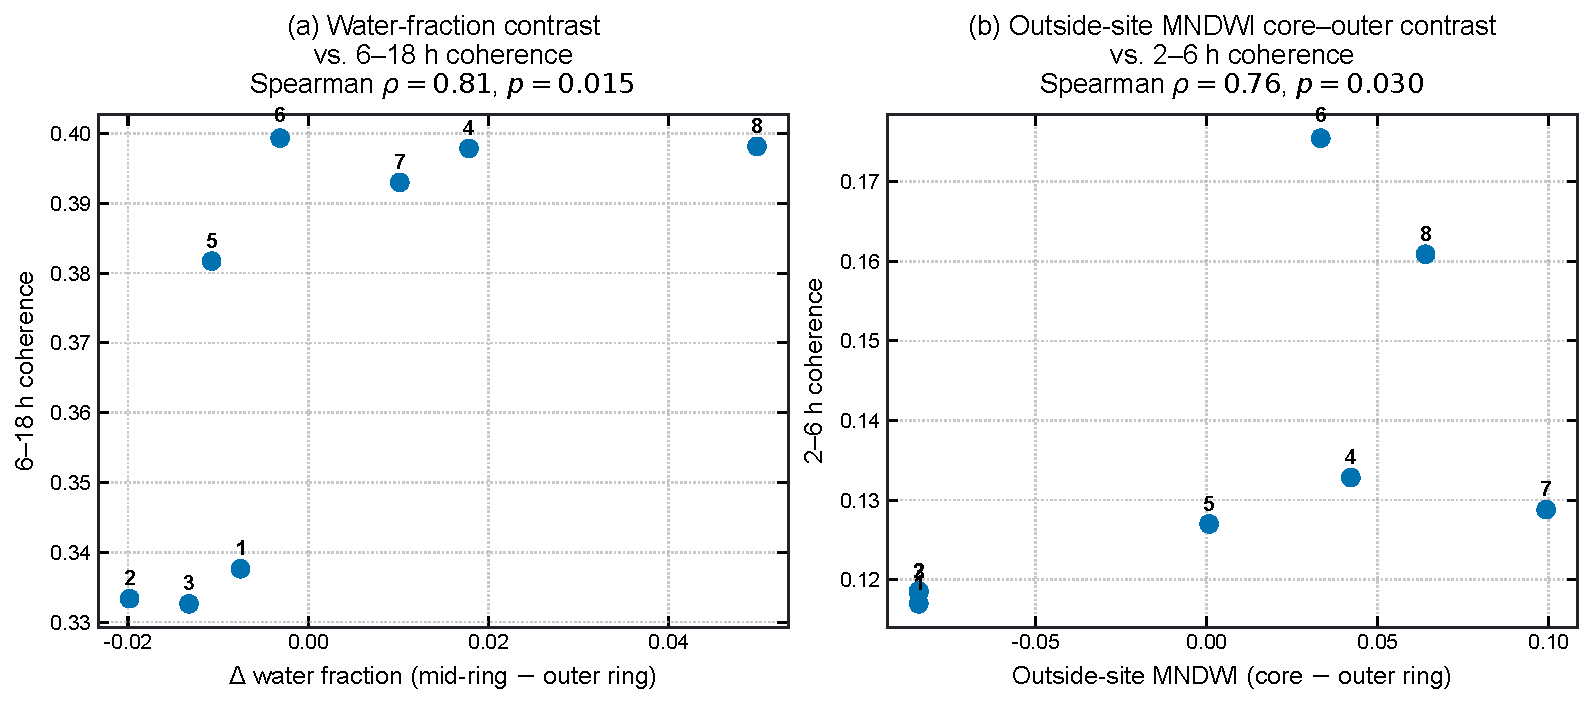
\includegraphics[width=\textwidth]{figures/Fig11_water_context_coherence_relationships_2021.pdf}
\caption{Water-context relationships with short-timescale wavelet coherence across the eight retained 2021 park--outside pairs. Panel (a) shows the leading water-fraction contrast relationship emphasized in the Results, while panel (b) shows a supporting outside-site moisture-index relationship. Each point is one retained park--outside pair, labeled numerically as follows: 1 = Chatuchak Park (Bang Sue), 2 = Wachirabenchathat Park (Bang Sue), 3 = Queen Sirikit Park (Bang Sue), 4 = Lumpini Park (Pathum Wan), 5 = Phra Nakhon Park (Lat Krabang), 6 = Nong Chok Park (Nong Chok), 7 = Seri Thai Park (Bueng Kum), and 8 = Suan Luang Rama IX (Prawet).}
\label{fig:water_context_coherence}
\end{figure}

The water layer therefore strengthened the explanatory analysis by adding a targeted coherence-oriented component beyond the vegetation and built-up gradients.

% [Figure 6 near here: top water relationships]
% [Table 4 near here: summary of strongest water-based correlations]

\subsection{Reviewed morphology contributes secondary support}

After polygon review and correction, morphology remained informative but clearly weaker than the land-cover and water layers. The strongest reviewed morphology signal was park perimeter, which showed a negative association with diurnal coherence ($\rho = -0.619$, $p = 0.102$). Park perimeter also showed negative associations with diurnal attenuation ($\rho = -0.595$, $p = 0.120$) and 2--6 h attenuation ($\rho = -0.595$, $p = 0.120$). Additional morphology features such as bounding-box fill ratio showed moderate but weaker associations, for example with diurnal coherence ($\rho = 0.548$, $p = 0.160$). None of the reviewed morphology relationships matched the strength of the leading annulus or water signals.

This result indicates that park shape alone did not dominate the attenuation--coherence patterns across the eight retained pairs. Instead, morphology functioned as a final, secondary explanatory layer that supported the broader spatial interpretation developed from the land-cover and water analyses. A cross-layer summary of the strongest explanatory associations is provided in Table~\ref{tab:top_explanatory_associations}.

\begin{table}[htbp]
\centering
\caption{Top explanatory associations across the four feature layers considered in this study. Rows summarize the strongest nonredundant feature--outcome relationships drawn from the mean-buffer, ring-gradient, water-context, and reviewed morphology scans. LOO range is reported only for the three leading mean-buffer relationships, for which leave-one-out robustness was explicitly evaluated.}
\label{tab:top_explanatory_associations}
\begingroup
\setlength{\tabcolsep}{3.6pt}
\renewcommand{\arraystretch}{1.12}
\scriptsize
\begin{tabular}{p{4.1cm}p{1.8cm}p{1.8cm}ccp{2.4cm}p{2.2cm}}
\toprule
Feature & Band & Outcome & Spearman $\rho$ & $p$-value & LOO range & Layer \\
\midrule
$\Delta$NDBI @ 250 m & 6--18 h & Attenuation & $+0.595$ & 0.120 & $+0.393$ to $+0.821$ & Mean buffer \\
$\Delta$NDBI @ 500 m & 7--14 d & Attenuation & $+0.595$ & 0.120 & $+0.393$ to $+0.786$ & Mean buffer \\
$\Delta$NDVI @ 500 m & 7--14 d & Attenuation & $-0.571$ & 0.139 & $-0.714$ to $-0.464$ & Mean buffer \\
Outside-site NDVI core $-$ outer & 2--6 h & Coherence & $-0.756$ & 0.030 & --- & Ring gradient \\
Outside-site NDBI core $-$ outer & 2--6 h & Coherence & $+0.708$ & 0.050 & --- & Ring gradient \\
$\Delta$NDBI in 250--500 m ring & 7--14 d & Attenuation & $+0.619$ & 0.102 & --- & Ring gradient \\
$\Delta$ water fraction (mid $-$ outer) & 6--18 h & Coherence & $+0.810$ & 0.015 & --- & Water context \\
Outside-site MNDWI core $-$ outer & 2--6 h & Attenuation & $+0.805$ & 0.016 & --- & Water context \\
Outside-site MNDWI core $-$ outer & 2--6 h & Coherence & $+0.756$ & 0.030 & --- & Water context \\
Park perimeter & 18--30 h & Coherence & $-0.619$ & 0.102 & --- & Morphology \\
\bottomrule
\end{tabular}
\endgroup
\end{table}
\section{Discussion} \subsection{Interpretation of the main wavelet findings} This study extends the interpretation of urban park air-quality effects beyond static inside--outside mean concentration differences by showing that Bangkok parks modify PM$_{2.5}$ variability in a strongly timescale-dependent manner. The wavelet attenuation--coherence framework reveals that parks do not simply reduce PM$_{2.5}$ by a fixed amount. Rather, they selectively damp particular temporal rhythms while still preserving part of the broader urban signal. In the present 2021 case study, damping was strongest and most consistent from sub-diurnal to multi-day scales, but the band structure was not monotonic: both the 2--6 h and diurnal bands were weaker, and the diurnal band showed the least damping overall. At the shortest 2--6 h band, a small number of parks even showed positive attenuation, indicating local amplification rather than damping at that timescale. This distinction matters scientifically and practically. A park that suppresses multi-day episode structure or sub-diurnal fluctuation amplitude is functioning differently from one that only marginally alters fast fluctuations or the daily cycle, even if their mean PM$_{2.5}$ values appear similar over time. The central methodological contribution of this study is therefore not just the use of continuous wavelet transform (CWT), but the pairing of attenuation and coherence as complementary descriptors of park buffering behavior. The regime concept is the key substantive novelty. The eight retained 2021 park--outside pairs did not behave as a single homogeneous class; instead, they organized naturally into strong decouplers, moderate broadband dampers, and weak followers or mixed cases. This shifts the framing of the urban-park question. Asking whether parks help with air quality is too blunt. The more useful question is which parks damp which temporal rhythms, how strongly they remain coupled to surrounding urban dynamics, and under what spatial conditions those behaviors emerge. In this sense, the regime classification is more informative than a citywide average effect size, because it respects internal heterogeneity among parks. It also provides a practical interpretation bridge between the spectral results and urban design: different park types may contribute differently to the buffering of short-term fluctuations, daily rhythms, or broader episode-scale variability. A stricter 14-day boundary-trim sensitivity check did not materially alter this qualitative three-regime structure, although some long-band attenuation magnitudes changed moderately. A second implication of the wavelet results is that amplitude damping and temporal coupling are not interchangeable concepts. From an exposure perspective, this means that a park may reduce the intensity of PM$_{2.5}$ episodes experienced inside the park even when the timing of broader urban pollution rhythms remains largely shared with the surrounding city. In practical terms, this kind of buffering may still be highly meaningful for public health and park use. Lowering the amplitude of daily or multi-day pollution fluctuations can reduce the severity of peak exposure conditions for park users even if the park does not become fully disconnected from city-scale atmospheric behavior. Thus, the value of a park as an air-quality buffer does not depend on becoming an isolated micro-atmosphere; it may instead lie in moderating the strength of pollution variability while remaining temporally embedded within the larger urban system. Two parks are especially revealing because they resist simplistic explanation. Nong Chok Park behaved as a strong decoupler despite not being reducible to a single mean greenness signal. This suggests that favorable spatial configuration, radial contrast structure, or local source separation may matter more than average vegetation alone. At the other end, Lumpini Park did not emerge as one of the strongest dampers despite its prominent green identity. This is a useful reminder that visual or intuitive greenness does not guarantee strong spectral damping performance. These cases strengthen, rather than weaken, the argument for a multi-factorial explanatory framework. They show why a one-variable interpretation would have been misleading and why the layered combination of mean land-cover contrast, ring gradients, water-related context, and morphology is more appropriate. \subsection{Spatial explanatory hierarchy} A major result of this study is that average greenness alone is not an adequate explanatory metric. The simple buffer-based results did show meaningful first-order relationships for park--outside NDVI and NDBI contrast, but these were not sufficient to explain the full hierarchy of damping behavior. The annulus-based analysis strengthened the interpretation considerably by showing that radial structure mattered more than mean composition alone. This is physically plausible. PM$_{2.5}$ attenuation is not expected to depend simply on whether vegetation is present, but on how it is organized: whether a protected vegetated interior exists, how quickly built-up pressure increases toward the edge, whether contrast persists outward from the park core, and how those transitions compare with the outside reference site. In that sense, the concepts of green-core advantage, built-edge pressure, and contrast persistence are not merely statistical labels; they are spatially intuitive descriptors of how a park is embedded within the surrounding urban fabric. Because NDVI and NDBI were extracted from station-centered buffers rather than clipped strictly to park boundaries, the built-up signal observed near park stations may reflect either internal hardscape or proximity to surrounding urban land cover, and these two contributions cannot be fully disentangled in the present dataset. The importance of ring-gradient structure also helps explain why the strongest explanatory signals often appeared for coherence, especially at short and sub-diurnal timescales. Short-band coherence reflects how tightly the park and outside station move together in time, even if their amplitudes differ. The finding that outside-site radial land-cover structure was strongly associated with short-band coherence suggests that local comparator context strongly influences whether a park remains dynamically synchronized with nearby urban fluctuations. This is a notable result because it shows that park performance is relational. A park is not acting in isolation; its apparent damping strength depends partly on what it is being compared against. If the outside site has a greener core, a sharper built-up edge, or a different water-related spatial organization, the inside--outside comparison itself changes in meaning. That outside-comparator insight is one of the most interesting findings of the study. Much of the literature implicitly treats the outside site as a neutral baseline, but the present results suggest that the baseline itself carries spatial structure that shapes the observed inside--outside relationship. This helps explain why some parks may appear to perform differently depending on their comparator context. It also means that future paired park studies should treat comparator selection as a substantive part of study design rather than as a purely technical detail. In the present workflow, the pairing was based on nearest geodesic distance under a transparent quality gate, which supports reproducibility. However, the results show that the spatial context of the outside site is not passive; it is an active part of the explanatory system. The role of water and morphology should be interpreted within that layered framework. Water-related metrics added a clear and targeted coherence-oriented signal, especially for short-band and 6--18 h synchrony, suggesting that moisture-sensitive local context may affect how quickly parks and outside sites respond together to changing conditions. However, water did not replace land-cover gradients as the dominant explanatory layer for attenuation across all bands. Morphology, even after reviewed polygon correction, remained secondary. This is an important negative result. It suggests that park footprint shape alone is not the primary control on PM$_{2.5}$ buffering behavior across this sample. In addition, the negative associations involving park perimeter should not be interpreted as evidence that greater edge exposure is beneficial. In this small sample, perimeter likely co-varies with park area and the existence of a larger protected vegetated core, so it is more plausibly acting as a partial size proxy than as a pure edge metric. Park form therefore becomes most meaningful when interpreted together with surrounding land-cover structure and comparator-site context. In other words, geometry matters, but not in isolation. Taken together, the explanatory hierarchy was clear. Mean land-cover contrast provided a useful first-order signal; annulus-based land-cover gradients provided the broadest explanatory improvement across attenuation and coherence; water-related context contributed some of the strongest individual associations, but in a narrower and more coherence-focused domain; and morphology offered secondary structural support. No single predictor explained all eight parks completely. Rather than a weakness, this is the result itself: PM$_{2.5}$ buffering by urban parks in Bangkok depends on a layered combination of internal green structure, surrounding built-up pressure, comparator-site context, water-related microenvironment, and park form. This layered explanatory hierarchy is synthesized conceptually in Fig.~\ref{fig:hierarchy_pyramid}. \begin{figure}[htbp]
\centering
\resizebox{\textwidth}{!}{%
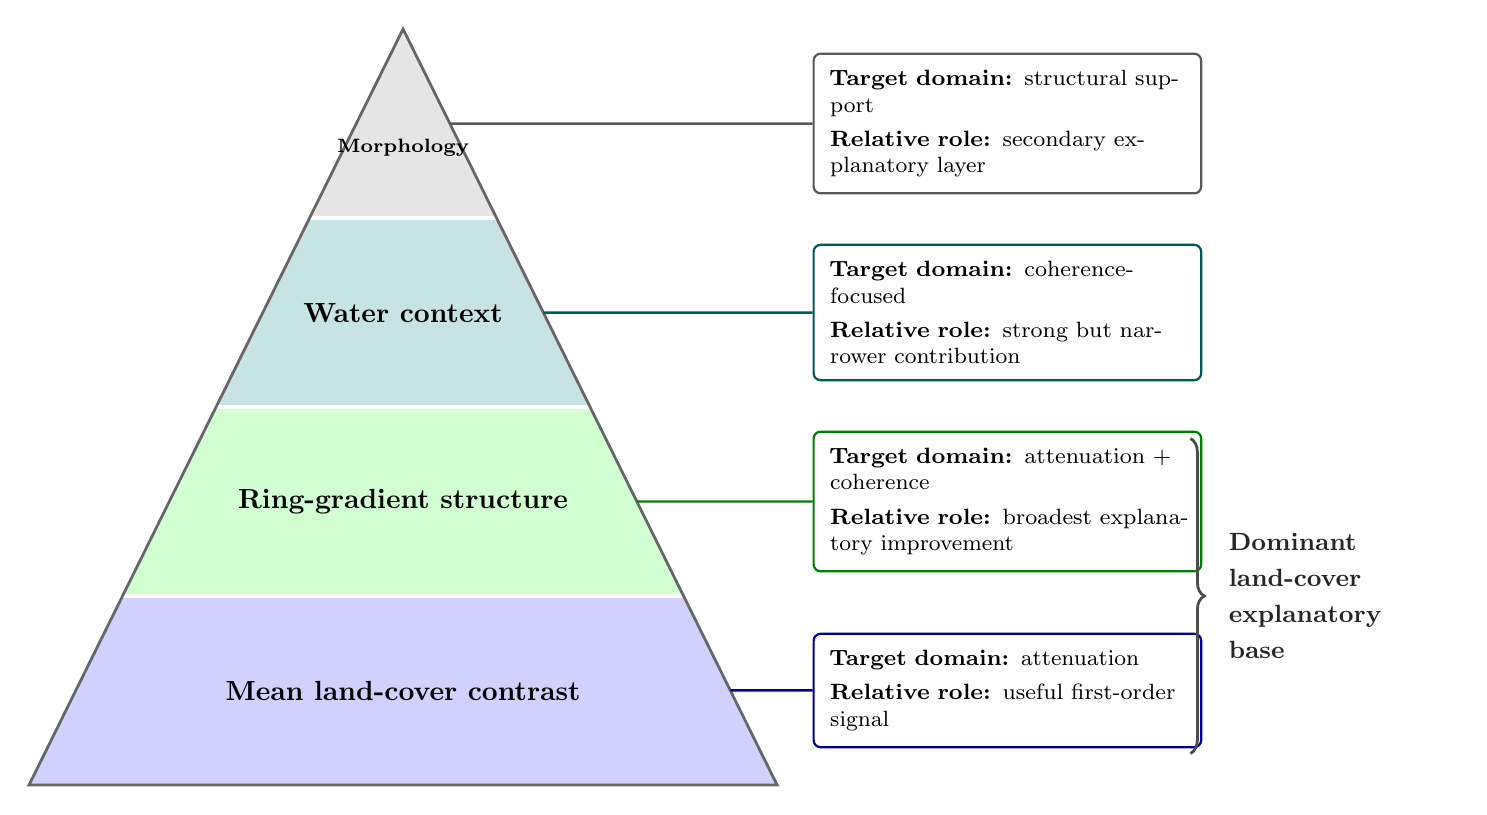
\begin{tikzpicture}[font=\sffamily]

% =========================
% Color Definitions
% =========================
\colorlet{col1}{blue!18}
\colorlet{col2}{green!18}
\colorlet{col3}{teal!22}
\colorlet{col4}{gray!20}

\colorlet{line1}{blue!60!black}
\colorlet{line2}{green!50!black}
\colorlet{line3}{teal!70!black}
\colorlet{line4}{gray!70!black}

% =========================
% Pyramid Geometry
% =========================
\def\W{9.5}   % Slightly widened base to easily fit the \normalsize text
\def\H{9.6}   % Total height
\def\CX{-3.0} % Center X of pyramid to balance the boxes on the right

\coordinate (BL) at (\CX-\W/2, 0);
\coordinate (BR) at (\CX+\W/2, 0);
\coordinate (TOP) at (\CX, \H);

% Y-coordinates of slice boundaries
\def\yA{2.4}
\def\yB{4.8}
\def\yC{7.2}

% Calculate coordinates on the edges
\coordinate (L1) at ($(BL)!\yA/\H!(TOP)$);
\coordinate (R1) at ($(BR)!\yA/\H!(TOP)$);
\coordinate (L2) at ($(BL)!\yB/\H!(TOP)$);
\coordinate (R2) at ($(BR)!\yB/\H!(TOP)$);
\coordinate (L3) at ($(BL)!\yC/\H!(TOP)$);
\coordinate (R3) at ($(BR)!\yC/\H!(TOP)$);

% =========================
% Filled layers & Borders
% =========================
\fill[col1] (BL) -- (BR) -- (R1) -- (L1) -- cycle;
\fill[col2] (L1) -- (R1) -- (R2) -- (L2) -- cycle;
\fill[col3] (L2) -- (R2) -- (R3) -- (L3) -- cycle;
\fill[col4] (L3) -- (R3) -- (TOP) -- cycle;

% Internal layer borders
\draw[white, line width=1.5pt] (L1) -- (R1);
\draw[white, line width=1.5pt] (L2) -- (R2);
\draw[white, line width=1.5pt] (L3) -- (R3);

% Outer pyramid border
\draw[black!60, line width=1pt] (BL) -- (BR) -- (TOP) -- cycle;

% =========================
% Box Styles
% =========================
\tikzset{
    infobox/.style={
        draw,
        rounded corners=2.5pt,
        line width=0.8pt,
        fill=white,
        align=left,
        text width=4.5cm,
        inner sep=6pt,
        font=\footnotesize % Reduced to standard diagram font size
    }
}

% =========================
% Edge Connectors & Boxes
% =========================
\coordinate (M1) at ($(BR)!0.5!(R1)$);
\coordinate (M2) at ($(R1)!0.5!(R2)$);
\coordinate (M3) at ($(R2)!0.5!(R3)$);
\coordinate (M4) at ($(R3)!0.5!(TOP)$);

\def\boxX{2.2} % Left edge of all boxes

% Box 1 (Mean)
\node[infobox, draw=line1] (box1) at (\boxX, 1.2) [anchor=west] {
    \textbf{Target domain:} attenuation\\[0.1cm]
    \textbf{Relative role:} useful first-order signal
};
\draw[line1, line width=0.9pt] (M1) -- (box1.west);

% Box 2 (Ring)
\node[infobox, draw=line2] (box2) at (\boxX, 3.6) [anchor=west] {
    \textbf{Target domain:} attenuation + coherence\\[0.1cm]
    \textbf{Relative role:} broadest explanatory improvement
};
\draw[line2, line width=0.9pt] (M2) -- (box2.west);

% Box 3 (Water)
\node[infobox, draw=line3] (box3) at (\boxX, 6.0) [anchor=west] {
    \textbf{Target domain:} coherence-focused\\[0.1cm]
    \textbf{Relative role:} strong but narrower contribution
};
\draw[line3, line width=0.9pt] (M3) -- (box3.west);

% Box 4 (Morphology)
\node[infobox, draw=line4] (box4) at (\boxX, 8.4) [anchor=west] {
    \textbf{Target domain:} structural support\\[0.1cm]
    \textbf{Relative role:} secondary explanatory layer
};
\draw[line4, line width=0.9pt] (M4) -- (box4.west);

% =========================
% Internal Pyramid Labels
% =========================
\node[font=\normalsize\bfseries] at (\CX, 1.2) {Mean land-cover contrast};
\node[font=\normalsize\bfseries] at (\CX, 3.6) {Ring-gradient structure};
\node[font=\normalsize\bfseries] at (\CX, 6.0) {Water context};
% Morphology is given a smaller font and lowered slightly to safely clear the borders
\node[font=\scriptsize\bfseries] at (\CX, 8.1) {Morphology};

% =========================
% Grouping Brace
% =========================
\draw[decorate,decoration={brace,amplitude=5pt,mirror},line width=1pt,black!70]
(7.0, 0.4) -- (7.0, 4.4)
node[midway, right=10pt, align=left, font=\small\bfseries, text width=2.8cm, color=black!85]
{Dominant\\[2pt]land-cover\\[2pt]explanatory\\[2pt]base};

\end{tikzpicture}%
}
\caption{Conceptual synthesis of the layered explanatory hierarchy identified in the Bangkok park--outside PM$_{2.5}$ wavelet analysis. Mean land-cover contrast provided a useful first-order signal, ring-gradient structure provided the broadest explanatory improvement across attenuation and coherence, water context contributed strong but narrower coherence-focused associations, and morphology acted as a secondary structural layer rather than a dominant control.}
\label{fig:hierarchy_pyramid}
\end{figure} \subsection{Implications for urban park design and management} Although the present analysis is exploratory and should not be interpreted as a direct intervention trial, the results do suggest several practical implications for urban park design and management in Bangkok. The first is that total green area alone is unlikely to be an adequate design target. The explanatory hierarchy developed here indicates that spatial organization matters at least as much as gross park area. In practical terms, parks with a more protected vegetated interior and lower central built-up pressure are likely to provide more favorable conditions for PM$_{2.5}$ damping than parks whose area is dominated by fragmented or edge-exposed green cover. A second implication is that the center of a park should be treated as a protected buffering zone rather than as the preferred location for extensive hardscape. The annulus-based results suggest that when built-up pressure penetrates toward the interior, the park loses part of its damping advantage. This does not mean that paved walkways, event spaces, or service infrastructure should be eliminated, but it does imply that large concrete plazas, wide paved corridors, or extensive impervious surfaces placed deep within the central zone may erode the function of the park as a PM$_{2.5}$ buffer. A more effective layout would place hardscape more selectively and preserve a comparatively uninterrupted interior vegetation core. A third implication concerns the park edge. The ring-gradient analysis indicates that transitions between the surrounding built environment and the park interior are highly relevant to buffering behavior. This suggests that the outer park zone should not be treated as a simple decorative boundary. Instead, boundary planting and edge design may be important for reducing direct penetration of nearby urban fluctuations into the interior. In practical planning terms, dense and vertically structured edge vegetation may be more valuable than sparse tree lines if the objective is to strengthen the contrast between the park interior and the surrounding street environment. A fourth implication concerns water features. In the present study, water-related metrics were most strongly associated with short-band and 6--18 h coherence rather than with universal broadband attenuation. This suggests that ponds, canals, or moisture-related landscape elements should not be treated as direct substitutes for vegetation, nor as simple particulate filters. However, the results are consistent with the possibility that water-sensitive local context helps stabilize short-timescale microenvironmental behavior and modifies the degree to which park and outside sites fluctuate together. In design terms, well-maintained water bodies may therefore contribute supportive microclimatic value when integrated with vegetation and favorable land-cover structure. A fifth implication is that park performance cannot be separated from the surrounding urban source environment. The relational importance of the outside comparator implies that heavy traffic, transport bottlenecks, or intense built-up pressure immediately adjacent to the park perimeter may overwhelm part of the park's buffering advantage. This is particularly relevant for cases such as Lumpini Park, where strong park identity does not automatically translate into the strongest damping regime. The practical lesson is that park design and traffic management should not be treated as independent policy domains. A park may perform better when perimeter traffic pressure, near-edge source density, and surrounding hardscape intensity are considered as part of the same environmental design problem. Taken together, these implications suggest a shift in planning emphasis: from maximizing green area in the abstract toward protecting vegetated cores, reducing central hardscape pressure, strengthening park-edge transitions, integrating supportive water context, and managing the immediate urban perimeter. These recommendations should be treated as design implications consistent with the present data, not as definitive prescriptions. However, they show how a wavelet-based, timescale-specific framework can be translated into concrete urban-management thinking more effectively than a static mean-concentration comparison alone. \subsection{Limitations and future directions} Several limitations should be stated explicitly. First, the effective sample size was small ($n = 8$ retained pairs), so all statistical relationships must be treated as exploratory. The Spearman and leave-one-out results are valuable as robustness-oriented pattern tests, but they do not support strong causal inference. Second, the paper is intentionally framed as a 2021 Bangkok case study. This is not because later years were ignored, but because 2022--2023 failed the same defensible annual quality gate, largely due to insufficient hourly completeness in the outside-station records. That decision strengthens the credibility of the paper, but it also means the conclusions should be interpreted as rigorously quality-gated for 2021 rather than as a multi-year climatology. Third, three parks shared the same outside comparator (Bang Sue District), which may have increased apparent similarity among some regime members and means that those parks should not be interpreted as fully independent confirmations of the same regime pattern. Fourth, the wavelet summaries compress behavior across a full year and therefore cannot resolve every local source event, directional transport pathway, or shifting meteorological regime within that window. Finally, the land-cover, water, and morphology features are correlative rather than causal. They identify spatial associations with damping behavior, but they do not, by themselves, prove mechanism. In addition, the main wavelet summaries were based on a fixed 24-h boundary trim rather than full scale-dependent cone-of-influence masking, so long-period attenuation estimates should be interpreted more cautiously than short-period or coherence-based results; a sensitivity check using a stricter 14-day trim changed some long-band attenuation magnitudes moderately, but the qualitative regime structure and the broader interpretation remained broadly consistent. These limitations point directly to future directions. The most immediate need is replication using denser and more stable monitoring networks with higher-quality outside comparators across multiple years. A second priority is the inclusion of directional or anisotropic spatial features, such as upwind--downwind sectors, because radial averages may miss important transport geometry. A third extension would be tighter integration with meteorological variables, especially wind speed, wind direction, atmospheric stability, and boundary-layer structure, which are likely to modulate when and how park damping becomes visible. A fourth future direction is application to other cities, where the same attenuation--coherence framework could test whether the Bangkok regime structure is generalizable or whether it depends on local urban morphology and climate. Despite these limitations, the broader implication is clear. Urban parks in Bangkok did not behave as interchangeable green spaces; they buffered PM$_{2.5}$ variability in different ways across timescales, and those differences were linked more strongly to layered spatial structure than to average greenness alone. The study therefore suggests that policy and design should move beyond the simple assumption that more green area automatically produces stronger air-quality benefits. Protected interior vegetation, reduced built-up edge pressure, and favorable spatial integration with surrounding urban land cover are likely to matter more than area alone. More broadly, the wavelet attenuation--coherence framework presented here offers a reproducible and transferable way to evaluate how urban green spaces interact with air-pollution dynamics in time, not just in mean concentration space.
\section{Conclusion}

This study developed a paired wavelet attenuation--coherence framework to evaluate timescale-specific PM$_{2.5}$ buffering by urban parks in Bangkok using defensible 2021 hourly park--outside station pairs. The central finding is that urban parks did not act as uniform mean-concentration reducers; rather, they modified PM$_{2.5}$ variability in distinct ways across timescales. Attenuation was negative overall, with the strongest damping generally occurring from sub-diurnal to multi-day bands, whereas coherence increased toward the diurnal and 2--7 d bands, indicating that parks often reduced fluctuation amplitude while remaining embedded within broader city-scale temporal rhythms.

A second key result is that Bangkok parks were not interchangeable. The retained pairs organized into three interpretable regimes---strong decouplers, moderate broadband dampers, and weak followers or mixed cases---showing that park air-quality function depends not only on whether variability is reduced, but also on how strongly park dynamics remain coupled to surrounding urban conditions. This makes the attenuation--coherence framework more informative than static inside--outside mean comparison alone.

The explanatory analysis further indicated that average greenness was not sufficient to explain this heterogeneity. Mean land-cover contrast provided a useful first-order signal, annulus-based land-cover gradients provided the broadest explanatory improvement, water-related context contributed strong but more targeted coherence-oriented associations, and reviewed morphology remained secondary. Together, these findings suggest that PM$_{2.5}$ buffering depends more on layered spatial structure---including protected vegetated interiors, surrounding built-up pressure, comparator-site context, and supportive local microenvironment---than on total green area alone.

From a practical perspective, the study suggests that urban park design should move beyond area-based greening targets and give greater attention to protected interior vegetation, reduced central hardscape pressure, stronger park-edge transitions, and the immediate surrounding urban perimeter. More broadly, the study provides a reproducible framework for evaluating how urban green spaces interact with air-pollution dynamics in time, not only in mean concentration space. The next priority is replication with denser multi-year monitoring and stronger directional context so that the Bangkok regime structure can be tested, refined, and translated more confidently into urban environmental design.

\section*{Software and analysis environment}
The main analysis was carried out in Python. Core packages included pandas, NumPy, matplotlib, SciPy, PyWavelets, GeoPandas, and Google Earth Engine for the remote-sensing feature extraction workflow.

\section*{Data availability}
Hourly PM$_{2.5}$ and meteorological observations were obtained from the Pollution Control Department (PCD), Ministry of Natural Resources and Environment (MONRE), Thailand, for Bangkok monitoring stations. Access to these data is subject to the policies of the data provider. Processed analysis outputs and derived summary tables used in this study are available from the author upon reasonable request.

\section*{Funding}
This research received no external funding.

\section*{Conflicts of interest}
The author declares no conflict of interest.

\bibliographystyle{apalike}
\bibliography{refs}

\end{document}